% I seguenti commenti speciali impostano:
% 1. 
% 2. PDFLaTeX come motore di composizione;
% 3. tesi.tex come documento principale;
% 4. il controllo ortografico italiano per l'editor.

% !TEX encoding = UTF-8
% !TEX TS-program = pdflatex
% !TEX root = tesi.tex
% !TEX spellcheck = it-IT

\documentclass[10pt,                    % corpo del font principale
               a4paper,                 % carta A4
               twoside,                 % impagina per fronte-retro
               openright,               % inizio capitoli a destra
               english,                 
               italian,                 
               ]{book}    

%**************************************************************
% Importazione package
%************************************************************** 

%\usepackage{amsmath,amssymb,amsthm}    % matematica

\usepackage[T1]{fontenc}                % codifica dei font:
                                        % NOTA BENE! richiede una distribuzione *completa* di LaTeX

\usepackage[utf8]{inputenc}             % codifica di input; anche [latin1] va bene
                                        % NOTA BENE! va accordata con le preferenze dell'editor

\usepackage[english, italian]{babel}    % per scrivere in italiano e in inglese;
                                        % l'ultima lingua (l'italiano) risulta predefinita

\usepackage{bookmark}                   % segnalibri

\usepackage{caption}                    % didascalie

\usepackage{chngpage,calc}              % centra il frontespizio

\usepackage{csquotes}                   % gestisce automaticamente i caratteri (")

\usepackage{emptypage}                  % pagine vuote senza testatina e piede di pagina

\usepackage{epigraph}			% per epigrafi

\usepackage{eurosym}                    % simbolo dell'euro

%\usepackage{indentfirst}               % rientra il primo paragrafo di ogni sezione

\usepackage{graphicx}                   % immagini

\usepackage{hyperref}                   % collegamenti ipertestuali

\usepackage[binding=5mm]{layaureo}      % margini ottimizzati per l'A4; rilegatura di 5 mm

\usepackage{listings}                   % codici

\usepackage{microtype}                  % microtipografia

\usepackage{mparhack,fixltx2e,relsize}  % finezze tipografiche

\usepackage{nameref}                    % visualizza nome dei riferimenti                                      

\usepackage[font=small]{quoting}        % citazioni

\usepackage{subfig}                     % sottofigure, sottotabelle

\usepackage[italian]{varioref}          % riferimenti completi della pagina

\usepackage[dvipsnames]{xcolor}         % colori

\usepackage{booktabs}                   % tabelle                                       
\usepackage{tabularx}                   % tabelle di larghezza prefissata                                    
\usepackage{longtable}                  % tabelle su più pagine                                        
\usepackage{ltxtable}                   % tabelle su più pagine e adattabili in larghezza

\usepackage[toc, acronym]{glossaries}   % glossario
                                        % per includerlo nel documento bisogna:
                                        % 1. compilare una prima volta tesi.tex;
                                        % 2. eseguire: makeindex -s tesi.ist -t tesi.glg -o tesi.gls tesi.glo
                                        % 3. eseguire: makeindex -s tesi.ist -t tesi.alg -o tesi.acr tesi.acn
                                        % 4. compilare due volte tesi.tex.

\usepackage[backend=biber,style=verbose-ibid,hyperref,backref]{biblatex}
                                        % eccellente pacchetto per la bibliografia; 
                                        % produce uno stile di citazione autore-anno; 
                                        % lo stile "numeric-comp" produce riferimenti numerici
                                        % per includerlo nel documento bisogna:
                                        % 1. compilare una prima volta tesi.tex;
                                        % 2. eseguire: biber tesi
                                        % 3. compilare ancora tesi.tex.

\usepackage[a-1b]{pdfx}

%**************************************************************
% file contenente le impostazioni della tesi
%**************************************************************

%**************************************************************
% Frontespizio
%**************************************************************

% Autore
\newcommand{\myName}{Alessandro Discalzi}                                    
\newcommand{\myTitle}{Advertising management system: Creazione e gestione di contenuti pubblicitari}

% Tipo di tesi                   
\newcommand{\myDegree}{Tesi di laurea}

% Università             
\newcommand{\myUni}{Università degli Studi di Padova}

% Facoltà       
\newcommand{\myFaculty}{Corso di Laurea in Informatica}

% Dipartimento
\newcommand{\myDepartment}{Dipartimento di Matematica "Tullio Levi-Civita"}

% Titolo del relatore
\newcommand{\profTitle}{Prof. }

% Relatore
\newcommand{\myProf}{Claudio Enrico Palazzi}

% Luogo
\newcommand{\myLocation}{Padova}

% Anno accademico
\newcommand{\myAA}{2019-2020}

% Data discussione
\newcommand{\myTime}{Settembre 2020}


%**************************************************************
% Impostazioni di impaginazione
% see: http://wwwcdf.pd.infn.it/AppuntiLinux/a2547.htm
%**************************************************************

\setlength{\parindent}{14pt}   % larghezza rientro della prima riga
\setlength{\parskip}{0pt}   % distanza tra i paragrafi


%**************************************************************
% Impostazioni di biblatex
%**************************************************************
\bibliography{bibliografia} % database di biblatex 

\defbibheading{bibliography} {
    \cleardoublepage
    \phantomsection 
    \addcontentsline{toc}{chapter}{\bibname}
    \chapter*{\bibname\markboth{\bibname}{\bibname}}
}

\setlength\bibitemsep{1.5\itemsep} % spazio tra entry

\DeclareBibliographyCategory{opere}
\DeclareBibliographyCategory{web}

\addtocategory{opere}{womak:lean-thinking}
\addtocategory{web}{site:agile-manifesto}

\defbibheading{opere}{\section*{Riferimenti bibliografici}}
\defbibheading{web}{\section*{Siti Web consultati}}


%**************************************************************
% Impostazioni di caption
%**************************************************************
\captionsetup{
    tableposition=top,
    figureposition=bottom,
    font=small,
    format=hang,
    labelfont=bf
}

%**************************************************************
% Impostazioni di glossaries
%**************************************************************

%**************************************************************
% Acronimi
%**************************************************************
\renewcommand{\acronymname}{Acronimi e abbreviazioni}

\newacronym[description={\glslink{apig}{Application Program Interface}}]
    {api}{API}{Application Program Interface}

\newacronym[description={\glslink{umlg}{Unified Modeling Language}}]
    {uml}{UML}{Unified Modeling Language}

%**************************************************************
% Glossario
%**************************************************************
%\renewcommand{\glossaryname}{Glossario}

\newglossaryentry{apig}
{
    name=\glslink{api}{API},
    text=Application Program Interface,
    sort=api,
    description={in informatica con il termine \emph{Application Programming Interface API} (ing. interfaccia di programmazione di un'applicazione) si indica ogni insieme di procedure disponibili al programmatore, di solito raggruppate a formare un set di strumenti specifici per l'espletamento di un determinato compito all'interno di un certo programma. La finalità è ottenere un'astrazione, di solito tra l'hardware e il programmatore o tra software a basso e quello ad alto livello semplificando così il lavoro di programmazione}
}

\newglossaryentry{umlg}
{
    name=\glslink{uml}{UML},
    text=UML,
    sort=uml,
    description={in ingegneria del software \emph{UML, Unified Modeling Language} (ing. linguaggio di modellazione unificato) è un linguaggio di modellazione e specifica basato sul paradigma object-oriented. L'\emph{UML} svolge un'importantissima funzione di ``lingua franca'' nella comunità della progettazione e programmazione a oggetti. Gran parte della letteratura di settore usa tale linguaggio per descrivere soluzioni analitiche e progettuali in modo sintetico e comprensibile a un vasto pubblico}
}

\newglossaryentry{systemIntegratorg}
{
    name=\glslink{System Integrator}{system integrator},
    text=System Integrator,
    sort=system Integrator,
    description=asd
}

\newglossaryentry{contenutog}
{
    name=\glslink{Contenuto informativo}{contenuto informativo},
    text=contenuti informativi,
    sort=contenuto informativo,
    description=asd
}

\newglossaryentry{cloudnativog}
{
    name=\glslink{Cloud nativo}{cloud nativo},
    text=Cloud nativo,
    sort=cloud nativo,
    description=asd
}

\newglossaryentry{appserverg}
{
    name=\glslink{Application server}{application server},
    text=Application server,
    sort=application server,
    description=asd
}

\newglossaryentry{microservizig}
{
    name=\glslink{Microservizi}{microservizi},
    text=Microservizi,
    sort=microservizi,
    description=asd
}

\newglossaryentry{iocg}
{
    name=\glslink{Inversione di controllo}{inversione di controllo},
    text=inversione di controllo,
    sort=inversione di controllo,
    description=asd
}

\newglossaryentry{dbmsg}
{
    name=\glslink{DBMS}{dbms},
    text=DBMS,
    sort=dbms,
    description=asd
}

\newglossaryentry{ui}
{
    name=\glslink{UI}{ui},
    text=UI,
    sort=ui,
    description=asd
}

\newglossaryentry{ux}
{
    name=\glslink{UX}{ux},
    text=UX,
    sort=ux,
    description=asd
}

\newglossaryentry{ci}
{
    name=\glslink{CI}{ci},
    text=CI,
    sort=ci,
    description=asd
}

\newglossaryentry{ssog}
{
    name=\glslink{SSO}{sso},
    text=SSO,
    sort=sso,
    description=asd
}

\newglossaryentry{mockg}
{
    name=\glslink{Mock}{mock},
    text=Mock,
    sort=mock,
    description=asd
} % database di termini
\makeglossaries


%**************************************************************
% Impostazioni di graphicx
%**************************************************************
\graphicspath{{immagini/}} % cartella dove sono riposte le immagini


%**************************************************************
% Impostazioni di hyperref
%**************************************************************
\hypersetup{
    %hyperfootnotes=false,
    %pdfpagelabels,
    %draft,	% = elimina tutti i link (utile per stampe in bianco e nero)
    colorlinks=true,
    linktocpage=true,
    pdfstartpage=1,
    pdfstartview=FitV,
    % decommenta la riga seguente per avere link in nero (per esempio per la stampa in bianco e nero)
    %colorlinks=false, linktocpage=false, pdfborder={0 0 0}, pdfstartpage=1, pdfstartview=FitV,
    breaklinks=true,
    pdfpagemode=UseNone,
    pageanchor=true,
    pdfpagemode=UseOutlines,
    plainpages=false,
    bookmarksnumbered,
    bookmarksopen=true,
    bookmarksopenlevel=1,
    hypertexnames=true,
    pdfhighlight=/O,
    %nesting=true,
    %frenchlinks,
    urlcolor=webbrown,
    linkcolor=RoyalBlue,
    citecolor=webgreen,
    %pagecolor=RoyalBlue,
    %urlcolor=Black, linkcolor=Black, citecolor=Black, %pagecolor=Black,
    pdftitle={\myTitle},
    pdfauthor={\textcopyright\ \myName, \myUni, \myFaculty},
    pdfsubject={},
    pdfkeywords={},
    pdfcreator={pdfLaTeX},
    pdfproducer={LaTeX}
}

%**************************************************************
% Impostazioni di itemize
%**************************************************************
\renewcommand{\labelitemi}{$\bullet$}

%**************************************************************
% Impostazioni di listings
%**************************************************************
\lstset{
    language=[LaTeX]Tex,%C++,
    keywordstyle=\color{RoyalBlue}, %\bfseries,
    basicstyle=\small\ttfamily,
    %identifierstyle=\color{NavyBlue},
    commentstyle=\color{Green}\ttfamily,
    stringstyle=\rmfamily,
    numbers=none, %left,%
    numberstyle=\scriptsize, %\tiny
    stepnumber=5,
    numbersep=8pt,
    showstringspaces=false,
    breaklines=true,
    frameround=ftff,
    frame=single
} 


%**************************************************************
% Impostazioni di xcolor
%**************************************************************
\definecolor{webgreen}{rgb}{0,.5,0}
\definecolor{webbrown}{rgb}{.6,0,0}


%**************************************************************
% Altro
%**************************************************************

\newcommand{\omissis}{[\dots\negthinspace]} % produce [...]

% eccezioni all'algoritmo di sillabazione
%*\hyphenation{}

\newcommand{\sectionname}{sezione}
\addto\captionsitalian{\renewcommand{\figurename}{Figura}
                       \renewcommand{\tablename}{Tabella}}

\newcommand{\glsfirstoccur}{\ap{{[g]}}}

\newcommand{\intro}[1]{\emph{\textsf{#1}}}

%**************************************************************
% Environment per ``rischi''
%**************************************************************
\newcounter{riskcounter}                % define a counter
\setcounter{riskcounter}{0}             % set the counter to some initial value

%%%% Parameters
% #1: Title
\newenvironment{risk}[1]{
    \refstepcounter{riskcounter}        % increment counter
    \par \noindent                      % start new paragraph
    \textbf{\arabic{riskcounter}. #1}   % display the title before the 
                                        % content of the environment is displayed 
}{
    \par\medskip
}

\newcommand{\riskname}{Rischio}

\newcommand{\riskdescription}[1]{\textbf{\\Descrizione:} #1.}

\newcommand{\risksolution}[1]{\textbf{\\Soluzione:} #1.}

%**************************************************************
% Environment per ``use case''
%**************************************************************
\newcounter{usecasecounter}             % define a counter
\setcounter{usecasecounter}{0}          % set the counter to some initial value

%%%% Parameters
% #1: ID
% #2: Nome
\newenvironment{usecase}[2]{
    \renewcommand{\theusecasecounter}{\usecasename #1}  % this is where the display of 
                                                        % the counter is overwritten/modified
    \refstepcounter{usecasecounter}             % increment counter
    \vspace{10pt}
    \par \noindent                              % start new paragraph
    {\large \textbf{\usecasename #1: #2}}       % display the title before the 
                                                % content of the environment is displayed 
    \medskip
}{
    \medskip
}

\newcommand{\usecasename}{UC}

\newcommand{\usecaseactors}[1]{\textbf{\\Attori Principali:} #1. \vspace{4pt}}
\newcommand{\usecasepre}[1]{\textbf{\\Precondizioni:} #1. \vspace{4pt}}
\newcommand{\usecasedesc}[1]{\textbf{\\Descrizione:} #1. \vspace{4pt}}
\newcommand{\usecasepost}[1]{\textbf{\\Postcondizioni:} #1. \vspace{4pt}}
\newcommand{\usecasealt}[1]{\textbf{\\Scenario Alternativo:} #1. \vspace{4pt}}

%**************************************************************
% Environment per ``namespace description''
%**************************************************************

\newenvironment{namespacedesc}{
    \vspace{10pt}
    \par \noindent                              % start new paragraph
    \begin{description} 
}{
    \end{description}
    \medskip
}

\newcommand{\classdesc}[2]{\item[\textbf{#1:}] #2}
                     % file con le impostazioni personali

\begin{document}
%**************************************************************
% Materiale iniziale
%**************************************************************
\frontmatter
% !TEX encoding = UTF-8
% !TEX TS-program = pdflatex
% !TEX root = ../tesi.tex

%**************************************************************
% Frontespizio 
%**************************************************************
\begin{titlepage}

\begin{center}

\begin{LARGE}
\textbf{\myUni}\\
\end{LARGE}

\vspace{10pt}

\begin{Large}
\textsc{\myDepartment}\\
\end{Large}

\vspace{10pt}

\begin{large}
\textsc{\myFaculty}\\
\end{large}

\vspace{29pt}
\begin{figure}[htbp]
\begin{center}

\includegraphics[height=6cm]{logo-unipd}
\end{center}
\end{figure}
\vspace{8pt} 

\begin{LARGE}
\begin{center}
\textbf{
    \begin{center}
        Advertising management system:
    \end{center} 
    Creazione e gestione di contenuti pubblicitari}\\
\end{center}
\end{LARGE}

\vspace{8pt} 

\begin{large}
\textsl{\myDegree}\\
\end{large}

\vspace{40pt} 

\begin{large}
\begin{flushleft}
\textit{Relatore}\\ 
\vspace{5pt} 
\profTitle \myProf
\end{flushleft}

\vspace{0pt} 

\begin{flushright}
\textit{Laureando}\\ 
\vspace{5pt} 
\myName
\end{flushright}
\end{large}

\vspace{40pt}

\line(1, 0){338} \\
\begin{normalsize}
\textsc{Anno Accademico \myAA}
\end{normalsize}

\end{center}
\end{titlepage} 
% !TEX encoding = UTF-8
% !TEX TS-program = pdflatex
% !TEX root = ../tesi.tex

%**************************************************************
% Colophon
%**************************************************************
\clearpage
\phantomsection
\thispagestyle{empty}

\hfill

\vfill

\noindent\myName: \textit{\myTitle,}
\myDegree,
\textcopyright\ \myTime.
%% !TEX encoding = UTF-8
% !TEX TS-program = pdflatex
% !TEX root = ../tesi.tex

%**************************************************************
% Dedica
%**************************************************************
\cleardoublepage
\phantomsection
\thispagestyle{empty}
\pdfbookmark{Dedica}{Dedica}

\vspace*{3cm}

\begin{center}
Lorem ipsum dolor sit amet, consectetuer adipiscing elit. \\ \medskip
--- Oscar Wilde    
\end{center}

\medskip

\begin{center}
Dedicato a ...
\end{center}

% !TEX encoding = UTF-8
% !TEX TS-program = pdflatex
% !TEX root = ../tesi.tex

%**************************************************************
% Sommario
%**************************************************************
\cleardoublepage
\phantomsection
\pdfbookmark{Sommario}{Sommario}
\begingroup
\let\clearpage\relax
\let\cleardoublepage\relax
\let\cleardoublepage\relax

\chapter*{Sommario}

Il presente documento descrive il lavoro svolto durante il periodo di stage dal laureando \myName presso l'azienda SCAI ITEC.
Lo stage è stato svolto al termine del percorso di studi della laurea triennale in informatica e la sua durata è stata di 312 ore.
L'obbiettivo dello stage è stato di implementare un applicativo per la creazione e per la gestione di contenuti pubblicitari.
Il presente documento vuole illustrare il contesto aziendale dove si è svolto lo stage, le attività svolte e una valutazione sul lavoro effettuato e su quanto appreso.

%\vfill
%
%\selectlanguage{english}
%\pdfbookmark{Abstract}{Abstract}
%\chapter*{Abstract}
%
%\selectlanguage{italian}

\endgroup			

\vfill


% !TEX encoding = UTF-8
% !TEX TS-program = pdflatex
% !TEX root = ../tesi.tex

%**************************************************************
% Ringraziamenti
%**************************************************************
\cleardoublepage
\phantomsection
\pdfbookmark{Ringraziamenti}{ringraziamenti}

\begin{flushright}{
	\slshape    
	``Nessuno ha mai ottenuto nulla con le lacrime.''} \\ 
	\medskip
    --- Brucaliffo
\end{flushright}


\bigskip

\begingroup
\let\clearpage\relax
\let\cleardoublepage\relax
\let\cleardoublepage\relax

\chapter*{Ringraziamenti}

\noindent \textit{Innanzitutto, vorrei esprimere la mia gratitudine al Prof. Claudio Enrico Palazzi, relatore della mia tesi, per l'aiuto e il sostegno che mi ha fornito durante la stesura del lavoro.}\\

\noindent \textit{Desidero ringraziare con affetto la mia famiglia, e in particolare i miei genitori per il sostegno e per il grande aiuto che mi hanno dato durante gli anni di studio.}\\

\noindent \textit{Desidero inoltre ringraziare il mio tutor aziendale, Dott. Bledar Gogaj, e il suo collega, Dott. Marco Lionello per l'enorme aiuto che mi hanno dato durante il periodo di stage.}\\

\noindent \textit{Un ringraziamento infine, ai miei amici per tutti i bei momenti passati insieme e per avermi sopportato tutti questi anni.}\\
\bigskip

\noindent\textit{\myLocation, \myTime}
\hfill \myName

\endgroup


% !TEX encoding = UTF-8
% !TEX TS-program = pdflatex
% !TEX root = ../tesi.tex

%**************************************************************
% Indici
%**************************************************************
\cleardoublepage
\pdfbookmark{\contentsname}{tableofcontents}
\setcounter{tocdepth}{2}
\tableofcontents
%\markboth{\contentsname}{\contentsname} 
\clearpage

\begingroup 
    \let\clearpage\relax
    \let\cleardoublepage\relax
    \let\cleardoublepage\relax
    %*******************************************************
    % Elenco delle figure
    %*******************************************************    
    \phantomsection
    \pdfbookmark{\listfigurename}{lof}
    \listoffigures

    \vspace*{8ex}

    %*******************************************************
    % Elenco delle tabelle
    %*******************************************************
    %\phantomsection
    %\pdfbookmark{\listtablename}{lot}
    %\listoftables
        
    \vspace*{8ex}
\endgroup

\cleardoublepage

\cleardoublepage

%**************************************************************
% Materiale principale
%**************************************************************
\mainmatter
% !TEX encoding = UTF-8
% !TEX TS-program = pdflatex
% !TEX root = ../tesi.tex

%**************************************************************
\chapter{Introduzione}
\label{cap:introduzione}
%**************************************************************

% Introduzione al contesto applicativo.\\

% \noindent Esempio di utilizzo di un termine nel glossario \\
% \gls{api}. \\

% \noindent Esempio di citazione in linea \\
% \cite{site:agile-manifesto}. \\

% \noindent Esempio di citazione nel pie' di pagina \\
%citazione\footcite{womak:lean-thinking} \\

%**************************************************************
\section{L'azienda}

\href{https://scaiitec.it/}{SCAI ITEC} è un'azienda italiana appartenente al \href{https://www.grupposcai.it/}{gruppo SCAI}. ITEC si occupa di consulenza, \textit{System Integration} e \textit{Application management} in ambito ICT. L'azienda opera principalmente in settore bancario, assicurativo, industriale e di pubblica amministrazione e servizi. \\Gli elementi chiave del successo e della crescita di SCAI ITEC sono:
\begin{itemize}
    \item vasta e profonda conoscenza delle tecnologie;
    \item grande attenzione per la soddisfazione del cliente;
    \item molta esperienza, maturata nel corso del tempo.
\end{itemize} 
ITEC è oggi una delle maggiori realtà nel nord-est del paese in ambito ICT e si propone come partner per qualsiasi tipo di applicazione, progetto e servizio modellato sulle specifiche necessità del cliente. 
\\Grazie alla consolidata esperienza nel ruolo di \textit{\gls{systemIntegratorg}\glsfirstoccur{}} e alle soluzioni \textit{leader} di mercato proposte, ITEC è in grado di garantire ai propri clienti risposte rapide, concrete e qualificate in base alle specifiche esigenze di tipo gestionale e applicativo.
\\Ultimo, ma non meno importante, dei motivi per cui l'azienda è all'avanguardia rispetto le nuove tecnologie è il grande investimento di ITEC in ricerca, sviluppo e formazione del personale.

\begin{figure}[h]
    \begin{center}
    
\includegraphics[width=0.5\textwidth]{logo-itec}
    \caption{Logo SCAI ITEC}
    \label{fig:figure1}
    \end{center}
\end{figure}


%**************************************************************
\section{Scopo dello stage}
\label{sez:scopo}
L'obiettivo principale dello stage è stato quello di inserire lo studente all'interno di una nuova progettualità, con un particolare \textit{focus} sulle tematiche legate alle tecnologie multimediali e alla loro distribuzione. Lo studente, affiancato da un \textit{IT Architect}, ha avuto la possibilità di partecipare al disegno, alla progettazione e realizzazione di una nuova progettualità. L'obiettivo è stato apprendere le tecnologie e le \textit{best practice} utilizzate in azienda, durante il ciclo di vita di un applicativo.
La progettualità vista è volta a creare un \textit{software} per la gestione di \gls{contenutog}\glsfirstoccur{}, per la loro creazione, modifica e distribuzione nei vari canali di vendita.
Grazie a questa nuova applicazione si potrà:
\begin{itemize}
    \item creare, modificare eliminare e clonare dei \gls{contenutog};
    \item raggruppare i \gls{contenutog} su segmenti di mercato e distribuirli;
    \item pianificare la visualizzazione e l’aggiornamento dei \gls{contenutog} sui vari canali di distribuzione;
    \item seguire un processo di \textit{Authoring} (paradigma Editore, Redattore, Supervisore) nella fase di creazione e distribuzione.
\end{itemize} 
In quanto l'intero progetto è di dimensione non indifferente l'obiettivo dello stage è stato di sviluppare le funzionalità relative al ruolo di editore, più nello specifico:
\begin{itemize}
    \item creazione di un contenuto;
    \item modifica di un contenuto;
    \item eliminazione di un contenuto;
    \item preparazione di un contenuto per la distribuzione;
    \item \textit{auditing} delle azioni effettuate dagli utenti;
    \item documentazione delle funzionalità implementate.
\end{itemize}

\section{Criticità e soluzioni}
Durante la pianificazione sono state evidenziate alcune criticità. Queste vengono descritte di seguito, insieme alle soluzioni trovate per mitigarle.

\subsection*{Conoscenza delle tecnologie}
Il progetto di stage prevedeva l'utilizzo di molteplici tecnologie mai utilizzate da me fino a quel momento. Questo ha introdotto il rischio di un eccessivo \textit{overhead} per l'apprendimento delle stesse. La soluzione adottata è stata la seguente:
\begin{itemize}
    \item ogni tecnologia mai utilizzata durante il mio percorso di studi è stata introdotta brevemente dal tutor aziendale;
    \item mi è stato fornito materiale da consultare per apprendere le basi delle nuove tecnologie;
    \item è stato infine deciso di utilizzare l'approccio \textit{"Learn by doing"} con la possibilità di chiedere aiuto al tutor aziendale nel caso fosse necessario.
\end{itemize} 

\subsection*{Coordinamento del team}
A causa del COVID-19 è stato deciso in comune accordo di svolgere il lavoro in modalità telematica per tutta la durata dello stage. Questo ha introdotto il rischio che ci fossero maggiorni difficoltà nelle interazioni con il tutor aziendale e il team di sviluppo. Tale rischio è stato mitigato grazie all'applicazione di \hyperref[sez:scrum]{Scrum}, che impone vengano effettuati dei meeting giornalieri per favorire il coordinamento del team.

\subsection*{Progettazione del database}
Uno dei momenti più importanti durante la fase di \hyperref[cap:analisi]{Analisi e Progettazione} è stata la progettazione della base di dati. Un'ideazione errata del \textit{database} avrebbe infatti introdotto numerosi problemi durante la codifica con il rischio di dover ripartire da zero nello sviluppo. Per mitigare tale rischio la base di dati una volta progettata è stata controllata attentamente da parte del tutor aziendale.

\section{Organizzazione del testo}

\begin{description}
    \item[{\hyperref[cap:obiettivi-pianificazione]{Il secondo capitolo}}] descrive gli obiettivi dello stage, la pianificazione del lavoro effettuata a monte e le aspettative personali riguardanti lo stage;
    
    \item[{\hyperref[cap:tecnologie]{Il terzo capitolo}}] descrive le tecnologie e gli strumenti di sviluppo utilizzati durante il corso dello stage;
    
    \item[{\hyperref[cap:metodologia-lavoro]{Il quarto capitolo}}] approfondisce la metodologia di lavoro e i ruoli adottati dal team di sviluppo;
    
    \item[{\hyperref[cap:analisi]{Il quinto capitolo}}] descrive l'analisi, la progettazione iniziale, e le soluzioni adottate durante la codifica;
    
    \item[{\hyperref[cap:prodotto]{Il sesto capitolo}}] descrive le funzionalità del prodotto finale, la documentazione e i test eseguiti;
    
    \item[{\hyperref[cap:considerazioni]{Il settimo capitolo}}] contiene le considerazioni finali riguardanti lo stage e una valutazione personale sul lavoro svolto;

\end{description}

Riguardo la stesura del testo, relativamente al documento sono state adottate le seguenti convenzioni tipografiche:
\begin{itemize}
	\item gli acronimi, le abbreviazioni e i termini ambigui o di uso non comune menzionati vengono definiti nel glossario, situato alla fine del presente documento;
	\item per la prima occorrenza dei termini riportati nel glossario viene utilizzata la seguente nomenclatura: \emph{parola}\glsfirstoccur{};
	\item i termini in lingua straniera o facenti parti del gergo tecnico sono evidenziati con il carattere \emph{corsivo}.
\end{itemize}             
% !TEX encoding = UTF-8
% !TEX TS-program = pdflatex
% !TEX root = ../tesi.tex

%**************************************************************
\chapter{Obbiettivi e pianificazione}
\label{cap:obbiettivi-pianificazione}
%**************************************************************

\intro{In questo capitolo sono descritti gli obbiettivi dello stage, la pianificazione del lavoro e le aspettative personali.}\\

%**************************************************************
\section{Obbiettivi}
L'obbiettivo di questo stage è la realizzazione di una \textit{Proof of Concept} dell'applicazione, in cui vengono rese disponibili le funzionalità descritte in \hyperref[sez:scopo]{§1.2}. Per aumentare la produttività e permettere allo studente di conoscere nuove tecnologie viene utilizzato \textit{\hyperref[jhi]{JHipster}}. Lo studente verrà inserito in un gruppo di lavoro composto da 4 persone in modo da favorire, oltre alla comprensione delle nuove tecnologie, la capacità di lavorare in un \textit{team}.
Al termine del periodo di stage verrà effettuata una presentazione del prodotto alla direzione dell'azienda.
\\Nel piano di lavoro, documento la cui stesura è avvenuta prima dell'inizio dello stage, sono stati individuati i seguenti obbiettivi suddivisi in obbligatori, desiderabili e opzionali.
\subsection{Obbiettivi obbligatori}
\begin{itemize}
    \item Ob1: Conoscenza del \textit{framework Spring} e in particolare \textit{Spring MVC REST};
    \item Ob2: Interazione e gestione \textit{database Oracle};
    \item Ob3: Realizzazione delle funzionalità \textit{backend} del progetto.
\end{itemize}
\subsection{Obbiettivi desiderabili}
\begin{itemize}
    \item D1: Realizzazione delle funzionalità \textit{frontend} del progetto;
    \item D2: Conoscenza base sviluppo applicazioni \textit{frontend Angular};
    \item D3: Grado di autonomia nel processo di analisi/sviluppo.
\end{itemize}
\subsection{Obbiettivi opzionali}
\begin{itemize}
    \item Op1: Conoscenza base dei strumenti per \textit{\gls{ci}\glsfirstoccur{}/\gls{cd}\glsfirstoccur{}}.
\end{itemize}

%**************************************************************
\section{Pianificazione}
Lo stage prevede una durata di 312 ore complessive corrispondenti a 8 ore di lavoro giornalierio per un periodo di circa 8 settimane. L'orario di lavoro è dal Lunedì al Venerdì, dalle ore 9:00 alle 13:00 e dalle ore 14:00 alle 18:00. L'ora tra le 13:00 e le 14:00 è dedicata alla pausa pranzo.
\\La pianificazione redatta per il periodo di stage, divisa per obbiettivi settimanali, è la seguente:
\begin{itemize}
    \item \textbf{prima settimana:}
    \begin{itemize}
        \item studio strumenti di sviluppo (\textit{Eclipse, Maven, Git});
        \item analisi dei requisiti.
    \end{itemize}
    \item \textbf{seconda settimana:}
    \begin{itemize}
        \item creazione struttura del \textit{database};
        \item gestione \textit{database Oracle}.
    \end{itemize}
    \item \textbf{terza settimana:}
    \begin{itemize}
        \item studio e utilizzo del \textit{framework Spring};
        \item studio e utilizzo di \textit{Hibernate};
        \item realizzazione dell'\textit{object-relational mapping}. 
    \end{itemize}
    \item \textbf{quarta settimana:}
    \begin{itemize}
        \item utilizzo \textit{spring MVC} e \textit{Jackson};
        \item realizzazione dei servizi \textit{REST}.
    \end{itemize}
    \item \textbf{quinta settimana:}
    \begin{itemize}
        \item studio e utilizzo di elementi avanzati di \textit{Oracle};
        \item gestione \textit{changeset Liquibase};
        \item sviluppo di altri servizi \textit{REST}. 
    \end{itemize}
    \item \textbf{sesta settimana:}
    \begin{itemize}
        \item studio di \textit{Angular};
        \item sviluppo \textit{frontend};
    \end{itemize}
    \item \textbf{settima settimana:}
    \begin{itemize}
        \item \textit{\gls{ci}} e \textit{\gls{cd}};
        \item utilizzo di \textit{Sonarqube};
        \item controllo qualità del codice.
    \end{itemize}
    \item \textbf{ottava settimana:}
    \begin{itemize}
        \item gestione \textit{cache} dell'applicazione;
        \item ottimizzazione;
    \end{itemize}
\end{itemize}

%**************************************************************
\section{Aspettative personali}
Le mie aspettative per quanto riguarda lo stage erano molteplici.
\\Prima tra tutte la possibilità di lavorare in un'azienda che produce \textit{software} in modo da poter capire, almeno in parte, come funziona la vita in azienda.
In secondo luogo il mio obbiettivo era quello di imparare nuove tecnologie e le \textit{best practice} adottate dall'azienda ospitante, anche grazie alla stretta collaborazione con il mio \textit{tutor}.
Ultima cosa ma non meno importante è la possibilità di farsi conoscere da un azienda leader nel settore, in modo da poter pensare a eventuali collaborazioni future.             
% !TEX encoding = UTF-8
% !TEX TS-program = pdflatex
% !TEX root = ../tesi.tex

%**************************************************************
\chapter{Tecnologie e strumenti di sviluppo}
\label{cap:tecnologie}

\intro{In questo capitolo sono descritte le tecnologie e gli strumenti di sviluppo utilizzati durante il corso dello stage.}\\

\section{Tecnologie}
\label{techs}

\subsection{JHipster}
\label{jhi}
\href{https://www.jhipster.tech/}{JHipster} è una piattaforma di sviluppo, con uno \textit{stack} tecnologico ben definito, utilizzata per generare, sviluppare e rilasciare, applicazioni e \textit{web services} all'avanguardia. Supporta molteplici tecnologie per il \textit{frontend}, tra le quali \textit{Angular}, \textit{React} e \textit{Vue}. Fornisce inoltre supporto per le applicazioni per dispositivi mobili utilizzando \textit{Ionic} e \textit{React Native}. Per quanto riguarda il \textit{backend}, JHipster supporta \textit{spring Boot} (con l'ausilio di \textit{Java} o \textit{Kotlin}), \textit{Micronaut}, \textit{Quarkus}, \textit{NodeJS} e \textit{.NET}. Per il rilascio sono adottati i principi di \gls{cloudnativog}\glsfirstoccur{}. Il rilascio è supportato su \textit{AWS}, \textit{Azure}, \textit{Cloud Foundry}, \textit{Google Cloud Platform}, \textit{Heroku} e \textit{OpenShift}.
\\L'obbiettivo di JHipster è generare applicazioni web o microservizi all'avanguardia, unendo:
\begin{itemize}
    \item uno \textit{stack} lato server robusto, ad alte prestazioni e coperto da test;
    \item un'interfaccia utente accattivante, moderna e \textit{mobile-first} usando \textit{Angular}, \textit{React} o \textit{Vue} e \textit{Bootstrap} per il \textit{CSS};
    \item un \textit{workflow} ben definito per fare la \textit{build} dell'applicazione con \textit{Maven} o \textit{Gradle};
    \item un'architettura a microservizi resiliente,  utilizzando i principi di \gls{cloudnativog};
    \item infrastruttura definita come codice, in modo da rendere la distribuzione su \textit{cloud} veloce.
\end{itemize}
\newpage
Nel corso dello stage JHipster è stato utilizzato per generare l'applicazione di base, utilizzata come punto di partenza per lo sviluppo.
\begin{figure}[h]
    \begin{center}
    
\includegraphics[width=0.18\textwidth]{logo-jhipster}
    \caption{Logo JHipster}
    \label{fig:figure2}
    \end{center}
\end{figure}

\subsection{Java Enterprise}
\href{https://www.oracle.com/it/java/technologies/java-ee-glance.html}{Java Enterprise}, conosciuto anche come \textit{Java EE} è un insieme di specifiche che mirano a estendere Java 8, aggiungendo funzionalità \textit{enterprise} come elaborazione distribuita e servizi web. Le applicazioni \textit{Java EE} possono essere eseguite sia come \gls{microservizig}\glsfirstoccur{} che su \gls{appserverg}\glsfirstoccur{}. In entrambi i casi vengono gestite: transazionalità, scalabilità, sicurezza e concorrenza.
Nel corso dello stage \textit{Java EE} è stato utilizzato per la programmazione lato \textit{backend}.
\begin{figure}[h]
    \begin{center}
    
\includegraphics[width=0.28\textwidth]{logo-javaee}
    \caption{Logo Java EE}
    \label{fig:figure3}
    \end{center}
\end{figure}

\subsection{Spring}
\href{https://spring.io/}{Spring} è un \textit{framework} applicativo \textit{open source} e un \textit{container} per l'\gls{iocg}\glsfirstoccur{} utilizzato dalla piattaforma \textit{Java}. Le funzionalità di base possono essere usate da una qualsiasi applicazione \textit{Java}, mentre quelle più avanzate sono disponibili solamente per \textit{Java Enterprise}.
Il \textit{framework Spring} ha a se associati vari moduli, nel corso del progetto sono stati utilizzati principalmente:
\begin{itemize}
    \item \textit{Spring Boot}: utilizzato per creare applicazioni basate su \textit{}, eseguibili senza la necessità di configurare un \textit{web server};
    \item \textit{Spring Data}: il cui obbiettivo è di facilitare la gestione e l'interazione di applicazioni \textit{Java} con un \textit{database}.
\end{itemize}
\begin{figure}[h]
    \begin{center}
    
\includegraphics[width=0.35\textwidth]{logo-spring}
    \caption{Logo Spring}
    \label{fig:figure4}
    \end{center}
\end{figure}

\subsection{Hibernate}
\href{https://hibernate.org/}{Hibernate} è un \textit{framework} per lo sviluppo di applicazioni in Java, utilizzato per gestire e mantenere su un \textit{database} relazionale un insieme di oggetti \textit{Java}.
\\Le sue funzionalità principali sono:
\begin{itemize}
    \item mappare oggetti \textit{Java} come tabelle su \textit{database};
    \item convertire i campi dati \textit{Java} a quelli del \gls{dbmsg}\glsfirstoccur{}{} utilizzato;
    \item generare chiamate \textit{SQL} e convertire la risposta ottenuta in un oggetto \textit{Java}.
\end{itemize}
Tali funzionalità sono state largamente utilizzate nel corso dello stage.
\begin{figure}[h]
    \begin{center}
    
\includegraphics[width=0.35\textwidth]{logo-hibernate}
    \caption{Logo Hibernate}
    \label{fig:figure5}
    \end{center}
\end{figure}

\subsection{REST}
\href{https://restfulapi.net/}{REST} è un modello architetturale per i sistemi distribuiti. I sistemi \textit{REST} si basano su \textit{HTTP} e prevedono una struttura degli \textit{URL} ben definita, che identifichi univocamente le risorse secondo la convenzione del modello stesso\footcite{Resource Naming: https://restfulapi.net/resource-naming/}. 
In \textit{REST} per il trasferimento di dati vengono utilizzati i metodi \textit{HTTP}, più nello specifico:
\begin{itemize}
    \item \textit{GET}: per il recupero di informazioni;
    \item \textit{POST, PUT, PATCH}: per l'inserimento di informazioni;
    \item \textit{DELETE}: per l'eliminazione di informazioni.
\end{itemize}
I principi guida di \textit{REST} sono:
\begin{itemize}
    \item \textit{client-server}: separazione dei problemi della \gls{ui}\glsfirstoccur da quelli di storage dei dati;
    \item \textit{statelessness}: ogni richiesta deve avere tutte le informazioni necessarie per il suo processamento;
    \item \textit{cacheable}: i client possono memorizzare in cache le risposte, queste devono essere definite esplicitamente o implicitamente \textit{cacheable}, in modo da evitare il riutilizzo di dati errati;
    \item \textit{uniform interface}: utilizzo di un'interfaccia di comunicazione omogenea tra \textit{client} e \textit{server} in modo da disaccoppiare e semplificare l'architettura per poterla modificare a blocchi;
    \item \textit{layered system}: la struttura del sistema può essere composta da strati gerarchici. In questo caso ogni componente non può "vedere" oltre lo strato con cui sta interagendo;
    \item \textit{code on demand(opzionale)}: il codice lato \textit{client} può essere esteso scaricando ed eseguendo \textit{applet} o \textit{script}.
\end{itemize}
Nella definizione di \gls{apig} se queste rispettano tutti i vincoli imposti dall'architettura \textit{REST} allora possono essere definite \textit{RESTful}.
\begin{figure}[h]
    \begin{center}
    
\includegraphics[width=0.2\textwidth]{logo-rest}
    \caption{Logo REST}
    \label{fig:figure6}
    \end{center}
\end{figure}

\subsection{Oracle}
\label{oracle}
\href{https://www.oracle.com/it/database/}{Oracle database} è un \gls{dbmsg} di tipo relazionale prodotto da \textit{\href{https://www.oracle.com/}{Oracle corporation}}. 
\\I \textit{database Oracle} sono noti per offrire \textit{performance}, scalabilità, affidabilità e sicurezza oltre a poter essere utilizzati sia \textit{on premise} che nel \textit{cloud}.
\begin{figure}[h]
    \begin{center}
    
\includegraphics[width=0.22\textwidth]{logo-oracle}
    \caption{Logo Oracle}
    \label{fig:figure7}
    \end{center}
\end{figure}

\subsection{Liquibase}
\href{https://www.liquibase.org/}{Liquibase} è una libreria \textit{open source} indipendente dal \gls{dbmsg} utilizzato. Durante il periodo di stage è stata utilizzata per tracciare, gestire e applicare le modifiche allo schema del \textit{database}.
\begin{figure}[h]
    \begin{center}
    
\includegraphics[width=0.23\textwidth]{logo-liquibase}
    \caption{Logo Liquibase}
    \label{fig:figure8}
    \end{center}
\end{figure}
\newpage
\subsection{Angular}
\href{https://angular.io/}{Angular} è un \textit{framework open source} per la progettazione e lo sviluppo di applicazioni web.
Le applicazioni \textit{Angular} vengono eseguite interamente lato \textit{client} ma grazie alla moltitudine di moduli presenti è possibile integrare un sistema di \textit{backend} più complesso eseguito lato \textit{server}.
Nel corso dello stage, il \textit{frontend}, è stato scritto interamente in \textit{Angular}.
\begin{figure}[h]
    \begin{center}
    
\includegraphics[width=0.23\textwidth]{logo-angular}
    \caption{Logo Angular}
    \label{fig:figure9}
    \end{center}
\end{figure}

%**************************************************************
\newpage
\section{Strumenti di sviluppo}
\label{strum}

\subsection{Eclipse}
\label{eclipse}
L'\textit{IDE} utilizzato per lo sviluppo, previo consiglio del \textit{tutor aziendale}, è stato \textit{\href{https://www.eclipse.org/}{Eclipse}}.
\textit{Eclipse} è un ambiente di sviluppo integrato multipiattaforma e rientra nella categoria di \textit{software} libero, distribuito secondo i termini della \textit{\href{https://www.eclipse.org/legal/epl-2.0/}{Eclipse Public License}}.
\begin{figure}[h]
    \begin{center}
    
\includegraphics[width=0.35\textwidth]{logo-eclipse}
    \caption{Logo Eclipse}
    \label{fig:figure10}
    \end{center}
\end{figure}

\subsection{Maven}
\label{maven}
\href{https://maven.apache.org/}{Maven} è uno strumento di gestione di progetti \textit{software}, è basato su un \textit{Project Object Model (POM)} e può gestire la \textit{build}, il \textit{reporting} e la documentazione di un progetto. Nel corso dello stage \textit{Maven} è stato utilizzato principalmente per automatizzare la \textit{build} del progetto, sia in sviluppo che in produzione.
\begin{figure}[h]
    \begin{center}
    
\includegraphics[width=0.3\textwidth]{logo-maven}
    \caption{Logo Maven}
    \label{fig:figure11}
    \end{center}
\end{figure}

\subsection{Git}
\label{git}
\href{https://git-scm.com/}{Git} è un sistema di controllo di versione distribuito, gratuito e \textit{open source}, progettato per gestire progetti di qualsiasi tipo. Nel corso dello stage l'utilizzo di \textit{Git} è stato affiancato a quello di \textit{GitLab}, una piattaforma web per la gestione di \textit{repository Git}.
\begin{figure}[h]
    \begin{center}
    
\includegraphics[width=0.2\textwidth]{logo-git}
    \caption{Logo Git}
    \label{fig:figure12}
    \end{center}
\end{figure}
\subsection{SQL Developer}
\href{https://www.oracle.com/database/technologies/appdev/sqldeveloper-landing.html}{SQL Developer} è un ambiente di sviluppo integrato per lavorare con \textit{SQL} nei \textit{database Oracle}. Nel corso dello stage è stato utilizzato per gestire e testare il \textit{database Oracle} usato in produzione.
\begin{figure}[h]
    \begin{center}
    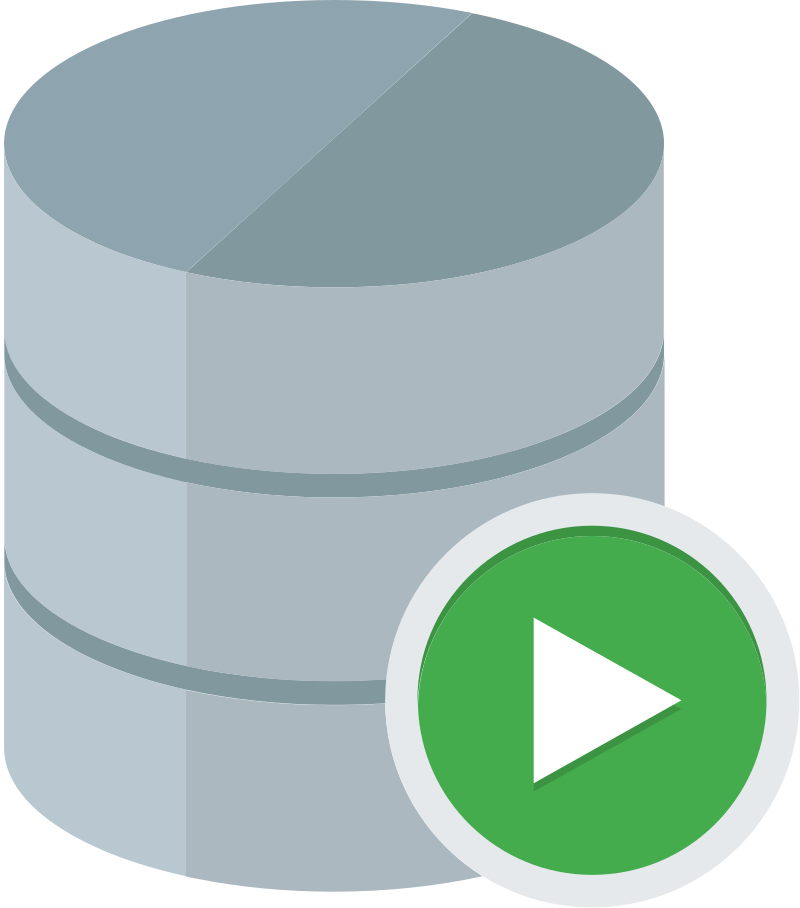
\includegraphics[width=0.18\textwidth]{logo-sqldeveloper}
    \caption{Logo SQL Developer}
    \label{fig:figure13}
    \end{center}
\end{figure}             
% !TEX encoding = UTF-8
% !TEX TS-program = pdflatex
% !TEX root = ../tesi.tex

%**************************************************************
\chapter{Metodologia di sviluppo}
\label{cap:metodologia-lavoro}
%**************************************************************

\intro{In questo capitolo viene descritta la metodologia di lavoro e i ruoli adottati dal \textit{team} di sviluppo.}\\

%**************************************************************
\section{Scrum}
\href{https://www.scrum.org/about}{\textit{Scrum}} è un \textit{framework} \textit{agile} per lo sviluppo, consegna e manutenzione di prodotti \textit{software} e non.
\textit{Scrum} è progettato per l'utilizzo in \textit{team} di dimensione ridotta. 
Di seguito vengono descritti ruoli, fasi e artefatti del \textit{framework}.

\subsection{Ruoli}

\subsubsection{Scrum Master}
Lo \textit{Scrum Master} aiuta il \textit{team} di sviluppo ad apprendere e applicare \textit{Scrum} per conseguire valore di \textit{business}. Lo \textit{Scrum Master} fa tutto ciò che è in suo potere per aiutare il \textit{team}, il \textit{Product Owner} e l'organizzazione ad avere successo. \textit{Scrum Master} non è il \textit{manager} dei membri del \textit{team}, né è un \textit{project manager}, \textit{team} \textit{leader}, o rappresentante del \textit{team}.
Lo scopo dello \textit{Scrum Master} è:
\begin{itemize}
    \item aiutare a rimuovere gli ostacoli durante lo sviluppo;
    \item evitare interferenze esterne;
    \item aiutare il \textit{team} ad adottare al meglio le pratiche di sviluppo \textit{agile};
    \item fare in modo che tutti applichino \textit{Scrum} nel miglior modo possibile.
\end{itemize}

\subsubsection{Product Owner}
Il \textit{Product Owner} ha la responsabilità di massimizzare il ritorno sugli investimenti (ROI), di identificare le caratteristiche del prodotto, traducendole in una lista di priorità, di decidere cosa dovrebbe andare in cima alla lista per il prossimo \textit{Sprint}, e di riassegnare le priorità, aggiornandole con continuità. Il \textit{Product Owner} detiene la responsabilità di profitto del prodotto, se questo è commerciale. In \textit{agile} il \textit{Product Owner} rappresenta il cliente e nell'applicazione di \textit{Scrum} può e deve:
\begin{itemize}
    \item definire il \textit{Product Backlog}, le \textit{user stories} e gli \textit{acceptance criteria};
    \item definire le priorità nel \textit{Product Backlog} e la data di rilascio del prodotto;
    \item accettare o rifiutare quanto sviluppato;
    \item cancellare lo \textit{Sprint} se risulta fallimentare o poco utile.
\end{itemize}


\subsubsection{Team di sviluppo}
Il \textit{team} di sviluppo è composto da un insieme di persone, in genere meno di dieci, e si occupa di sviluppare quanto definito dal \textit{Product Owner}. Il \textit{team} \textit{Scrum} deve essere \textit{"cross-funzionale"}, ovvero includere tutte le competenze necessarie allo sviluppo del prodotto. I membri del \textit{team} devono essere proattivi e aperti allo studio di tecnologie che vanno oltre le loro competenze.
Il \textit{team} di sviluppo:
\begin{itemize}
    \item costruisce il prodotto definito dal \textit{Product Owner};
    \item possiede tutte le conoscenze per ottenere un prodotto potenzialmente rilasciabile alla fine di ogni \textit{Sprint};
    \item è auto organizzato, con un alto grado di autonomia e responsabilità;
    \item decide quanti e quali elementi del \textit{Product Backlog} sviluppare;
    \item ha la responsabilità di sviluppo, \textit{test} e rilascio del prodotto;
    \item non possiede un \textit{team} \textit{leader}, in quanto in \textit{Scrum} nel \textit{team} di sviluppo sono considerati tutti di pari livello.
\end{itemize}

Nel corso dello stage i ruoli erano così suddivisi:
\begin{itemize}
    \item \textit{scrum master}: Bledar Gogaj
    \item \textit{team} di sviluppo: Alessandro Discalzi, Tania Parolin
    \item \textit{product owner}: Marco Lionello
\end{itemize}

\subsection{Artefatti}

\subsubsection{Product Backlog}
Il \textit{Product Backlog} è un elenco di funzionalità, centrate sul cliente e ordinato per priorità, esiste e si evolve per tutta la durata del prodotto. Il \textit{Product Backlog} definisce quindi tutto ciò che deve essere fatto ed include una moltitudine di voci, più nello specifico:
\begin{itemize}
    \item nuove funzionalità da implementare;
    \item obbiettivi di miglioramento;
    \item lavori di ricerca;
    \item difetti da risolvere, se in numero contenuto;
\end{itemize}
Un buon \textit{Product Backlog} è \textit{\textbf{DEEP}}:
\begin{itemize}
    \item \textbf{dettagliato}, con maggior attenzione alle voci di priorità più alta;
    \item \textbf{stimato}: per ogni voce deve esserci una stima per il completamento, la stima viene definita dal \textit{team} di sviluppo;
    \item \textbf{emergente}: il \textit{Product Backlog} viene aggiornato in base alla variabilità del progetto;
    \item \textbf{prioritizzato}: le voci sono ordinate per priorità, quelle con priorità più alta forniscono maggior valore al prodotto.
\end{itemize}
Nel corso del progetto di stage per gestire il \textit{Product Backlog} è stato utilizzato \textit{\href{https://taiga.io/}{Taiga}}, un tool per la gestione di progetti \textit{agile}.
\begin{figure}[h]
    \begin{center}
    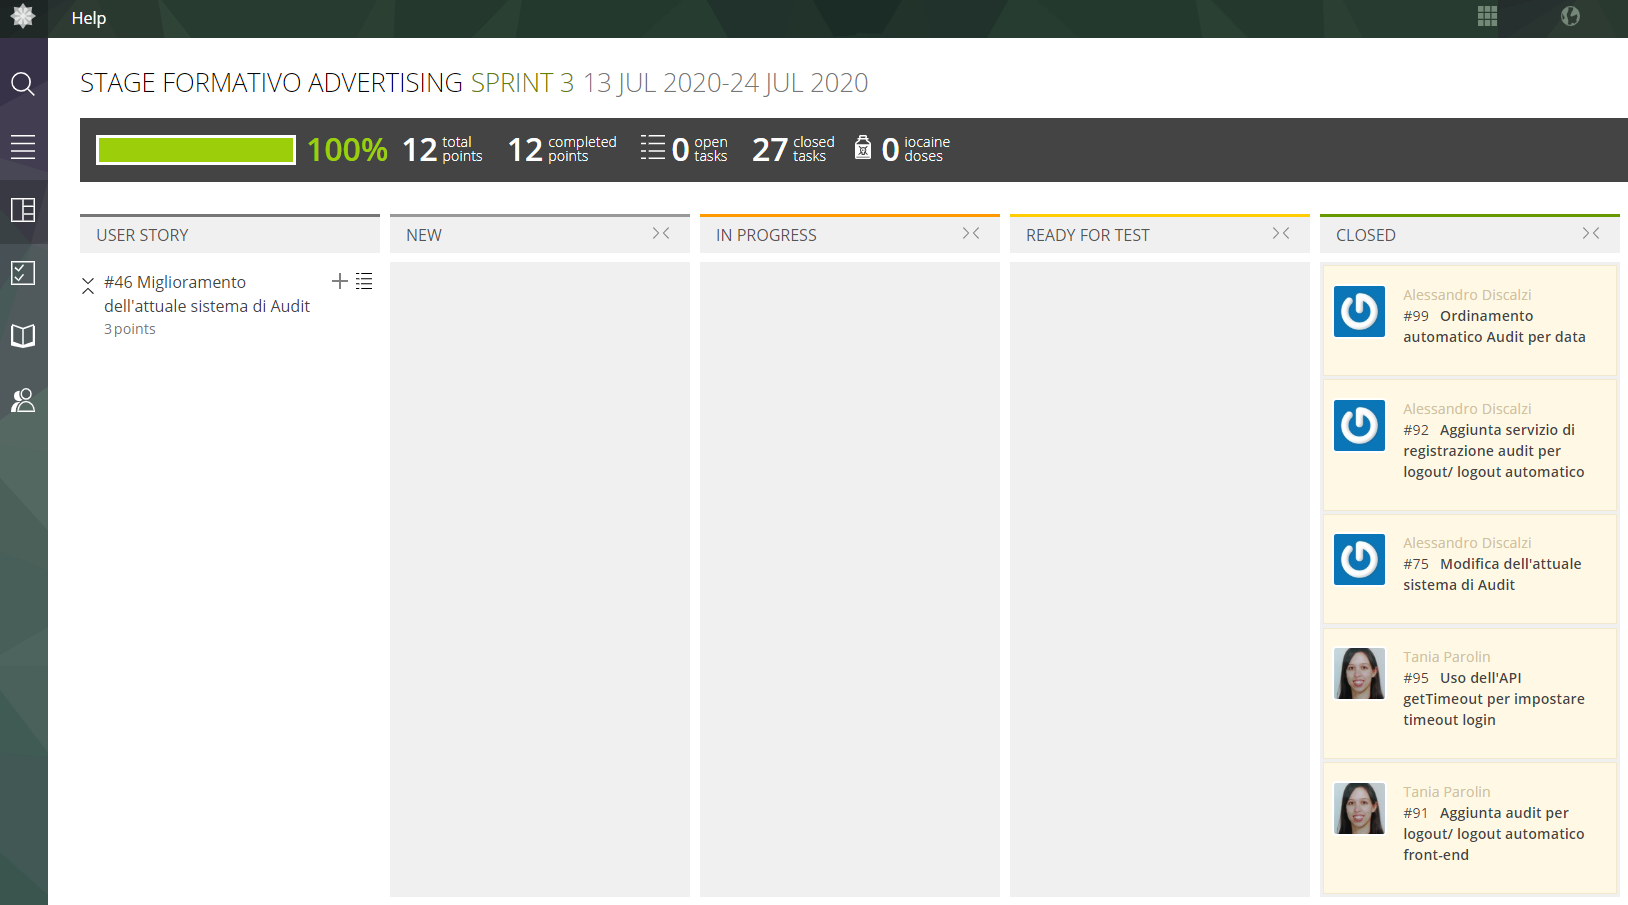
\includegraphics[width=1.2\textwidth]{taiga}
    \caption{Screenshot del backlog presente su Taiga rispetto uno degli \textit{Sprint} terminati}
    \label{fig:figure14}
    \end{center}
\end{figure}
\\Nel \textit{Product Backlog} di AMS la lista delle attività eseguite, in ordine di priorità, è la seguente:
\begin{itemize}
    \item \textit{design} e realizzazione della base di dati;
    \item \textit{design} e realizzazione del template di base per i contenuti pubblicitari;
    \item realizzazione della funzione di \textit{preview} di un contenuto;   
    \item gestione autenticazione e autorizzazione in base ai ruoli;
    \item realizzazione dei servizi di \textit{back-end}; 
    \item \textit{design} e implementazione della \gls{ui}\glsfirstoccur{};
    \item integrazione \textit{front-end} e \textit{back-end};
    \item implementazione della creazione di nuovi contenuti;
    \item implementazione della modifica di un contenuto;
    \item miglioramento \gls{ux}\glsfirstoccur{} e \gls{ui};
    \item inizio stesura documentazione;
    \item implementazione sistema di \textit{auditing};
    \item miglioramento dei contenuti di esempio;
    \item predisposizione di \textit{Oracle};
    \item implementazione \textit{breadcrumbs};
    \item aggiunta controlli di validazione;
    \item completamento della documentazione;
    \item controlli sull'accessibilità del \textit{software};
    \item miglioramento pipeline di \gls{ci}\glsfirstoccur{};
    \item predisposizione demo.
\end{itemize}

\subsubsection{Definition of done}
Durante ogni \textit{Sprint} ciò che viene fatto costituisce un prodotto potenzialmente rilasciabile, questo deve essere approvato dal \textit{Product Owner}, dallo \textit{Scrum Master} e dal \textit{team} di sviluppo prima dell'inizio dello \textit{Sprint} successivo. La \textit{definition of done} è un insieme di regole che definiscono quando ciò che viene fatto può essere definito rilasciabile.
La \textit{definition of done} adottata durante lo stage è la seguente:
\begin{itemize}
    \item AMS (Advertising Management System) deve essere stato compilato senza \textit{warning};
    \item il \textit{software} deve essere stato deployato nell’ambiente locale senza l'introduzione di nuovi errori e/o \textit{warning};
    \item devono essere stati eseguiti i \textit{test} sulle nuove funzionalità;
    \item il codice deve essere stato revisionato dallo \textit{Scrum Master}/\textit{Product Owner};
    \item la \textit{feature} implementata deve essere accettata dal \textit{Product Owner}.
\end{itemize}
Nei casi in cui questa definizione non fosse applicabile (ad esempio nel caso di modifiche che richiedono più voci/\textit{user stories}/\textit{Sprint}) avrebbe dovuto essere evidenziata la violazione del \textit{Definition of Done} allo \textit{Scrum Master} e al \textit{Product Owner} ritardando la chiusura del \textit{Done} a quando fosse stato effettivamente possibile.



\subsection{Fasi}

\subsubsection{Sprint}
Uno \textit{Sprint} è un periodo di tempo ben definito, di solito due settimane o un mese, durante il quale il \textit{team} di sviluppo completa una parte di lavoro in base a quanto definito nel \textit{Product Backlog}.
Gli \textit{Sprint} hanno durata fissa che non può essere estesa, tuttavia se lo \textit{Sprint} risulta fallimentare od obsoleto può essere cancellato prima del termine dal \textit{Product Owner}.
\\Nel corso del progetto didattico la durata degli \textit{Sprint} è stata fissata a due settimane, mentre la durata e gli argomenti discussi durante le riunioni descritte successivamente hanno seguito le regole di \textit{Scrum}.

\subsubsection{Sprint planning}
Lo \textit{Sprint} \textit{planning} è un incontro che viene effettuato prima di ogni \textit{Sprint}, la cui durata è limitata a due ore per ogni settimana di \textit{Sprint}. L'obbiettivo dello \textit{Sprint} \textit{planning} è definire cosa rilasciare al termine del prossimo \textit{Sprint} e come farlo.
Il lavoro da fare viene selezionato dal \textit{Product Backlog} e inserito nello \textit{Sprint} anche in base alle stime di completamento definite dal \textit{team} di sviluppo.

\subsubsection{Daily scrum}
Il Daily \textit{Scrum} è una delle pratiche chiave di \textit{Scrum}. Si tratta di un meeting giornaliero, della durata massima di quindici minuti, a cui partecipa il \textit{team} di sviluppo, lo \textit{Scrum Master} e, se richiesto, il \textit{Product Owner}. Il \textit{Daily} \textit{Scrum} serve a sincronizzare il \textit{team} e durante questo ogni membro deve rispondere a tre domande:
\begin{itemize}
    \item cosa è stato fatto dall'ultima riunione?
    \item cosa sarà fatto prima della prossima riunione?
    \item quali difficoltà si sono incontrate?
\end{itemize}
Nel caso alcuni ostacoli necessitino di discussioni approfondite queste possono essere fatte al termine del \textit{Daily} \textit{Scrum}.

\subsubsection{Sprint review}
La \textit{Sprint} review si tiene alla fine di uno \textit{Sprint}, in modo da ispezzionare gli incrementi e aggiornare, se necessario, il \textit{Product Backlog} di conseguenza. Durante la \textit{Sprint} review il \textit{team} di lavoro e gli \textit{stakeholders} collaborano per vedere, in base a quanto fatto durante lo \textit{Sprint}, quali sono le prossime cose che si potrebbero fare per aumentare il valore del prodotto. La \textit{Sprint} review dura massimo un'ora per ogni settimana di \textit{Sprint}, durante la riunione si svolgono le seguenti attività:
\begin{itemize}
    \item il \textit{Product Owner} spiega quali attività del \textit{backlog} sono state fatte e quali no;
    \item il \textit{team} di sviluppo discute di cosa è andato bene, di cosa è andato storto e di come si sono affrontati i problemi durante lo \textit{Sprint};
    \item il \textit{team} di sviluppo mostra il lavoro fatto e risponde ad eventuali domande riguardo l'incremento;
    \item se necessario il \textit{Product Owner} decide le date di rilascio in base a quanto fatto;
    \item il gruppo di lavoro collabora per decidere cosa fare prossimamente, questo serve anche come input allo \textit{Sprint} planning;
    \item \textit{review} del potenziale di mercato del prodotto, se il prodotto è commerciale.
\end{itemize}

\subsubsection{\textit{Sprint} retrospective}
La \textit{Sprint} retrospective ha luogo dopo la \textit{Sprint} review e prima dello \textit{Sprint} \textit{planning} e la sua durata è limitata a quarantacinque minuti per ogni settimana di \textit{Sprint}. Durante la retrospettiva, che viene vista come una possibilità di miglioramento per il \textit{team}, si discute di cosa è andato bene, di cosa è andato storto e di come si può migliorare per il prossimo \textit{Sprint}. Questo favorisce il \textit{team} in quanto si possono migliorare le metodologie adottate nello \textit{Sprint} precedente in base a ciò che è andato storto.             
% !TEX encoding = UTF-8
% !TEX TS-program = pdflatex
% !TEX root = ../tesi.tex

%**************************************************************
\chapter{Analisi e progettazione}
\label{cap:analisi}
%**************************************************************

\intro{Il seguente capitolo descrive l'analisi, la progettazione iniziale, e le soluzioni addottate durante la codifica}\\


%**************************************************************
\section{Analisi e progettazione iniziale}
Le funzionalità da implementare e gli obiettivi da raggiungere erano già ben definiti all'inizio del progetto, in quanto l'analisi funzionale è stata fornita dal \textit{product owner} insieme a una prima definizione del \textit{product backlog}.
Per questo motivo la fase di analisi dei requisiti da parte del \textit{team} di sviluppo è stata molto breve e si è concentrata principalmente su come le funzionalità del prodotto dovessero essere fruibili all'utente finale. La progettazione del \textit{software} non è avvenuta solamente all'inizio, ma si è protratta durante tutto il periodo di stage. Questo ha garantito maggior flessibilità nell'implementazione delle funzionalità e ha favorito l'utilizzo di Scrum. Tale scelta tuttavia ha anche introdotto il rischio che una debole progettazzione iniziale potesse causare problemi nelle settimane a venire. Questo rischio è stato subito mitigato grazie ad un attenta progettazione della base di dati pensando, nel miglior modo possibile, alle entità, a come esse fossero in relazione tra di loro e alla logica necessaria per implementare le funzionalità richieste. Inoltre, in quanto \textit{JHipster} utilizza uno \textit{stack} tecnologico ben definito, e impone dei vincoli architetturali da seguire, tale rischio è ulteriormente ridotto poiché non è necessario progettare l'architettura del \textit{software}.
Nel corso di questo capitolo vengono descritte le principali attività di progettazione svolte durante il corso dello stage.

%**************************************************************
\section{Progettazione del database}
La progettazione del \textit{database} è stata una delle attività più importanti, deteneva infatti un alto grado di priorità anche nel \textit{product backlog}. La progettazione del \textit{database} è stata divisa in due parti: la prima mirata a individuare le entità partendo dall'analisi dei requisiti fatta dal \textit{product owner}, mentre la seconda mettendo in relazione tali entità e aggiungendo tabelle se necessario. Per quanto riguarda la vera e propria implementazione del \textit{database} è stato sfruttato un tool fornito da \textit{JHipster} ovvero \href{https://start.JHipster.tech/jdl-studio/}{JDL-Studio}, che verrà descritto in modo dettagliato successivamente nel corso di questa sezione.

\subsection{Entità}
Durante la progettazione della base di dati sono state definite le entità descritte di seguito.
Per ciascuna di esse viene riportata una breve descrizione e la lista dei campi dati corredata dal tipo di dato. Nella lista seguente non vengono riportate chiavi primarie ne chiavi esterne poiché l'inserimento di tali campi dati è automatizzato e verrà descritto dettagliatamente nella sezione relativa alle \hyperref[rel]{relazioni tra entità}.
Mentre si stava effettuando la progettazione del \textit{database} è sorto il problema di come si volessero salvare i \gls{contenutog} e i \textit{template}. Si è optato di suddividere i contenuti in pagine, ognuna delle quali può contenere uno o più elementi multimediali e/o testuali. Inoltre in uno stesso contenuto si può selezionare un \textit{template} diverso per ogni pagina. Per quanto riguarda i \textit{template}, i quali sono definiti a monte dal \textit{team} di sviluppo, si è scelto di strutturarli definendo un \textit{template} al cui interno sono contenuti vari item che possono essere sia testuali che multimediali. Questo rende tutto il più modulare possibile, in quanto non pone limiti né in fase di creazione di un contenuto, né nella definizione dei \textit{template} e nel loro utilizzo. 
\subsubsection{Content}
Definisce un contenuto informativo, i suoi campi dati sono:
\begin{itemize}
    \item \textit{name (String)}: Nome del contenuto;
    \item \textit{state (State)}: Enumerazione che definisce i possibili stati di un contenuto;
    \item \textit{description (String)}: descrizione del contenuto informativo;
    \item \textit{slideTime (Integer)}: durata delle slide di un contenuto;
\end{itemize}

\subsubsection{ContentPage}
Definisce una pagina inserita in un contenuto. Ogni contenuto può avere più pagine che scorrono come slide durante la visualizzazione dello stesso; ogni pagina contiene degli item multimediali o testuali. I suoi campi dati sono:
\begin{itemize}
    \item \textit{pageNumber (Integer)}: numero della pagina all’interno di un contenuto.
\end{itemize}

\subsubsection{MultimediaItem}
Definisce un item multimediale (immagine o video) contenuto in una pagina. I suoi campi dati sono:
\begin{itemize}
    \item \textit{path (String)}: percorso del file multimediale caricato sul server, nel caso il caricamento delle immagini avvenga su NAS;
    \item \textit{resolution (Resolution)}: enumerazione che definisce la risoluzione dell'immagine caricata;
    \item \textit{multimediaFile (Blob)}: file multimediale caricato su \textit{database}, nel caso il caricamento non avvenga su NAS;
\end{itemize}

\subsubsection{TextItem}
Definisce un testo contenuto in una pagina. I suoi campi dati sono:
\begin{itemize}
    \item \textit{text (Blob)}: contenuto testuale inserito in una pagina.
\end{itemize}

\subsubsection{Template}
Definisce un \textit{template} che utilizzabile dalle pagine di un contenuto. Ogni pagina può utilizzare \textit{template} definiti a monte che determinano come immagini, video e contenuti testuali vengono disposti nella pagina al momento della presentazione. I suoi campi dati sono:
\begin{itemize}
    \item \textit{previewImage (Blob)}: immagine di preview del \textit{template}, utilizzata per aiutare l'utente a capire come questo è definito;
    \begin{figure}[h]
        \begin{center}
        
\includegraphics[width=0.18\textwidth]{textImage50_50}
        \caption{Immagine di preview di un \textit{template} contenente un testo e un'immagine}
        \label{fig:figure15}
        \end{center}
    \end{figure}
    \item \textit{templateHTML (Blob)}: contiene l'html del \textit{template};
    \item \textit{name (String)}: Nome del \textit{template}.
\end{itemize}

\subsubsection{TemplateItem}
Definisce un \textit{item} all'interno di un \textit{template}. Per \textit{item} si intende un singolo testo, immagine o video. Questa entità viene utilizzata in fase di creazione e di visualizzazione di un contenuto ed è utilizzata per sapere cosa va inserito in una pagina che utilizza un determinato \textit{template}. 
I suoi campi dati sono:
\begin{itemize}
    \item \textit{description (String)}: descrizione dell'item del \textit{template} (e.g. video a schermo intero);
    \item \textit{type (itemType)}: enumerazione che definisce il contenuto che viene inserito in quell’area del \textit{template};
    \item \textit{templateArea (Integer)}: area del \textit{template} in cui un certo oggetto va inserito, utilizzato in fase di preview per inserire immagini, video e testi al posto giusto all'interno del \textit{template}.
\end{itemize}

\subsubsection{CSS}
Definisce il CSS utilizzato da uno o più \textit{template}. I suoi campi dati sono:
\begin{itemize}
    \item \textit{templateCSS (Blob)}: contiene il CSS utilizzato da uno o più \textit{template}.
\end{itemize}

\subsubsection{CustomAudit}
Entità definita per implementare il sistema di Audit. I suoi campi dati sono:
\begin{itemize}
    \item \textit{action (Action)}: enumerazione che definisce il tipo di azione registrata negli audit;
    \item \textit{description (String)}: descrizione dettagliata dell'azione effettuata;
    \item \textit{timestamp (Instant)}: data e ora in cui l'azione registrata è stata eseguita.
\end{itemize}

\subsubsection{User}
Entità predefinita in \textit{JHipster} contenente tutte le informazioni necessarie per registrare un utente. Per utilizzarla è sufficiente definire relazioni ad essa.

\subsection{Enumerazioni}
Durante la progettazione della base di dati, in alcuni casi, si è ritenuto necessario definire alcuni campi dati come enumerazione al posto di utilizzare una semplice stringa di testo.
Questo garantisce maggior controllo e impone vincoli che evitano il verificarsi di errori relativi all'utilizzo di nomi diversi per esprimere lo stesso concetto. Le enumerazioni definite durante la progettazione del \textit{database} sono le seguenti.

\subsubsection{State}
Lista dei possibili stati di un contenuto informativo, ovvero: \textit{CREATED, TO\textunderscore{}ASSOCIATE, ASSOCIATED, TO\textunderscore{}AUTHORIZE, AUTHORIZED, PUBLISHED}.

\subsubsection{Resolution}
Lista delle possibili risoluzioni di un elemento multimediale, ovvero: \textit{HIGH, MEDIUM, LOW}.

\subsubsection{ItemType}
Lista delle diverse tipologie di \textit{template} item, ovvero: \textit{IMAGE, VIDEO, TEXT}.

\subsubsection{Action}
Lista delle azioni da registrare nel sistema di auditing che possono essere effettuate da un utente, ovvero: \textit{CREATE, DELETE, UPDATE, AUTHENTICATION\textunderscore{}SUCCESS, AUTHENTICATION\textunderscore{}FAILURE, LOGOUT, TIMEOUT}.

\subsection{Relazioni}
\label{rel}
Di seguito vengono evidenziate le relazioni tra le entità descritte in precedenza e ne viene data una breve descrizione.
\subsubsection{Content-ContentPage}
Ogni \textit{Content} può avere una o più \textit{ContentPage}, ogni \textit{ContentPage} è inserita in un solo contenuto.
\subsubsection{Template-ContentPage}
Ogni \textit{template} può essere utilizzato da una o più \textit{ContentPage}, ogni \textit{ContentPage} utilizza un solo \textit{template}.
\subsubsection{ContentPage-MultimediaItem}
Ogni \textit{ContentPage} può contenere uno o più \textit{MultimediaItem}, ogni \textit{MultimediaItem} è contenuto in una sola pagina.
\subsubsection{ContentPage-TextItem}
Ogni \textit{ContentPage} può contenere uno o più \textit{TextItem}, ogni \textit{TextItem} è contenuto in una sola pagina.
\subsubsection{Template-TemplateItem}
Ogni \textit{template} ha al suo interno uno o più \textit{templateItem}, ogni \textit{templateItem} fa riferimento a un solo \textit{template}.
\subsubsection{MultimediaItem-TemplateItem}
Ogni \textit{MultimediaItem} può riferirsi ad un solo \textit{templateItem}, ad ogni \textit{templateItem} possono essere riferiti uno o più \textit{MultimediaItem}.
\subsubsection{TextItem-TemplateItem}
Ogni \textit{TextItem} può riferirsi ad un solo \textit{templateItem}, ad ogni \textit{templateItem} possono essere riferiti uno o più \textit{TextItem}.
\subsubsection{Content-User}
Ogni \textit{Content} è creato da un solo \textit{User}, ogni \textit{User} può creare uno o più \textit{content}.
\subsubsection{CSS-template}
Ogni \textit{template} può avere uno o più \textit{CSS}, ogni \textit{CSS} può essere utilizzato da uno o più \textit{template}.
\subsubsection{CustomAudit-User}
Ogni \textit{Audit} si riferisce ad un solo \textit{User}, ad ogni \textit{User} possono essere registrati uno o più \textit{Audit}.


\subsection{Implementazione}
\subsubsection{JDL-Studio}
\textit{JDL-Studio} è un \textit{tool} fornito da \textit{JHipster} che permette di definire lo schema entità-relazioni di un \textit{database} tramite un apposito linguaggio di \textit{scripting} chiamato, appunto, \textit{JDL}. Una delle funzionalità più utili di \textit{JDL-Studio} è la possibilità di visualizzare il modello ER, che viene automaticamente aggiornato a ogni modifica.
\newpage
\subsubsection{Definizione di un'entità in JDL-Studio}
Un'entità viene definita in \textit{JD}L specificando il suo nome e i suoi campi dati. Un esempio di definizione di un'entità è il seguente:
\begin{lstlisting}[caption={Definizione entità Content},label={lst:ent}]
entity Content {
  name String unique,
  state State,
  description String,
  slideTime Integer
}
\end{lstlisting}
\subsubsection{Definizione di un'enumerazione in JDL-Studio}
Un'enumerazione viene definita in \textit{JDL} specificandone il nome e i suoi possibili valori dati. Un esempio di definizione di un'entità è il seguente:
\begin{lstlisting}[caption={Definizione enumerazione State},label={lst:en}]
enum State {
  CREATED,
  TO_ASSOCIATE,
  ASSOCIATED,
  TO_AUTHORIZE,
  AUTHORIZED,
  PUBLISHED
}
\end{lstlisting}
\subsubsection{Definizione di una relazione in JDL-Studio}
Per definire una relazione in \textit{JDL} bisogna innanzitutto specificare il tipo di relazione (uno a uno, uno a molti, molti a molti). Fatto questo è sufficiente specificare l'entità di partenza della relazione e quella di arrivo. Un esempio di definizione di relazioni in \textit{JDL} è il seguente:
\begin{lstlisting}[caption={Definizione relazioni uno a molti},label={lst:rel}]
    relationship OneToMany {
        Content{page} to ContentPage{content},
        Template{page} to ContentPage{template},
        ContentPage{multimediaItem} to MultimediaItem{page},
        TemplateItem{multimediaItem} to MultimediaItem{templateItem},
        Template{templateItem} to TemplateItem{template},
        ContentPage{textItem} to TextItem{page},
        TemplateItem{textItem} to TextItem{templateItem}
      }
\end{lstlisting}
\newpage
\subsubsection{Modello ER}
Il modello ER autogenerato presenta imperfezioni nella visualizzazione delle relazioni, nonostante ciò e stato ritenuto sufficiente per gli scopi del progetto.
\begin{figure}[h]
    \begin{center}
    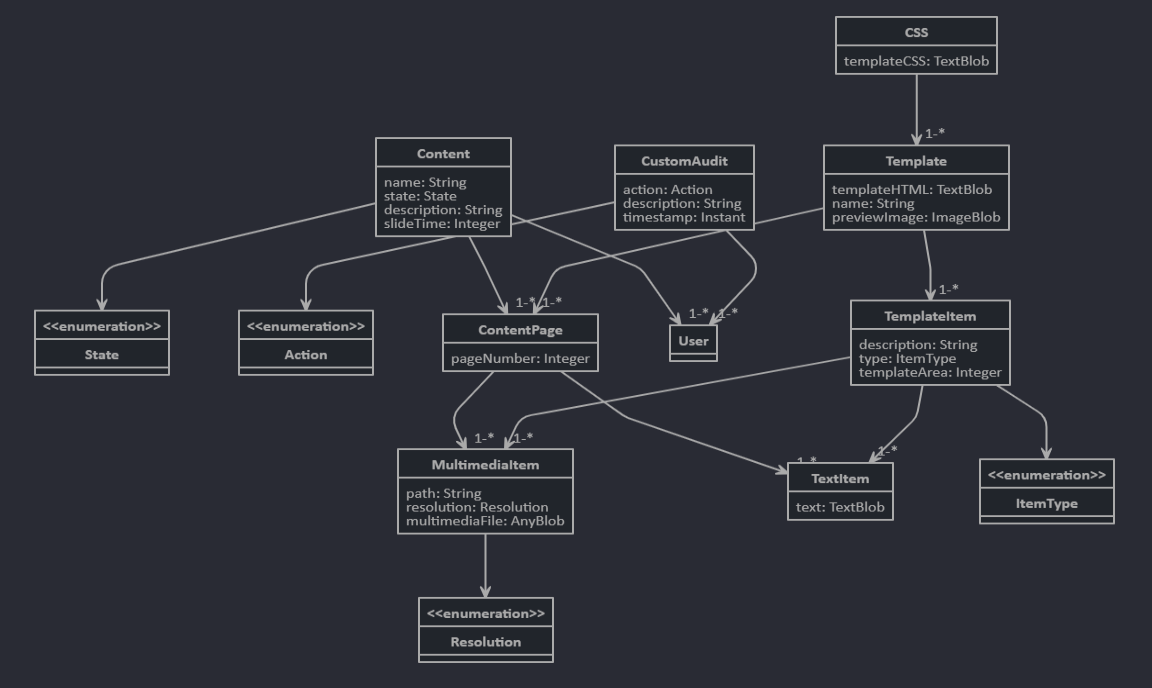
\includegraphics[width=1.2\textwidth]{er}
    \caption{Modello ER generato da JDL-Studio}
    \label{fig:figure19}
    \end{center}
\end{figure}
\\Una volta creato il modello del \textit{database} tramite \textit{JDL-Studio} è possibile importarlo direttamente all'interno dell'applicativo.
Tale procedura oltre a generare il \textit{database} crea anche una struttura di base dell'applicazione completa di \textit{back-end} e \textit{front-end}. Seppur questa non risulta completa di tutte le funzionalità necessarie, evita la scrittura di numerose linee di codice al programmatore riducendo l'introduzione di errori umani.
%**************************************************************
\section{Definizione dei template per i contenuti}
In quanto nella progettazione del \textit{database} è stato scelto di modellare i \textit{template} in modo che fossero più modulari ed estendibili possibile, è stata necessaria un'accurata definizione degli stessi. Si è optato per definire un \textit{template} di base utilizzato da ciascun contenuto informativo, e una serie di \textit{template} personalizzati utilizzati dalle pagine inserite in un contenuto.
\subsection{Template di base}
Il \textit{template} di base definito contiene poche informazioni. Definisce infatti la struttura base della pagina \textit{html} e la funzione per visualizzare le \textit{slide}. Contiene inoltre vari \textit{placeholder} utilizzati per inserire dinamicamente le informazioni di un determinato contenuto informativo.
I placeholder definiti sono: 
\begin{itemize}
    \item \textit{\$\{CSS\}}: Utilizzato per inserire il \textit{CSS} dei \textit{template} utilizzati;
    \item \textit{\$\{CONTENTID\}}: Utilizzato per inserire l’identificativo del contenuto come campo \textit{id} nel codice \textit{html};
    \item \textit{\$\{PAGES\}}: Utilizzato per inserire le pagine presenti in un contenuto;
    \item \textit{\$\{SLIDETIME\}}: Utilizzato per impostare lo slidetime scelto in un contenuto;
\end{itemize}
\subsection{Template di pagina}
I \textit{template} di pagina sono quelli scelti dall'utente durantela creazione di un contenuto.
Anche in questo caso i \textit{template}, scritti in \textit{html}, avranno al loro interno opportuni \textit{placeholder} per inserire i dati al momento dell'utilizzo. Poiché non si può sapere a priori come saranno definiti i \textit{template} futuri sono state definite delle regole da seguire durante la creazione di un nuovo \textit{template}. La lista delle regole definite è la seguente:
\begin{itemize}
    \item definire un nome del \textit{template} univoco;
    \item anteporre il nome del \textit{template} ad ogni classe o \textit{id} utilizzati per il \textit{CSS};
    \item non definire \textit{CSS} per gli elementi \textit{html} (e.g. H1, div, p), definirlo solamente classi e \textit{id};
    \item definire un tag \textit{<div>...</div>} differente per ogni \textit{item} del \textit{template};
    \item nel caso si volessero inserire video o immagini all'interno di un nuovo \textit{template} seguire gli esempi forniti insieme alla documentazione;
    \item definire i placeholder per l'inserimento di video, immagini o elementi testuali nel formato \textit{\$\{ItemType\textit{template}Area\}};
\end{itemize}

%**************************************************************
\section{Definizione dei servizi di back-end}
Durante l'importazione del modello del \textit{database} \textit{JHipster} genera automaticamente alcuni servizi \textit{RESTful} per ciascuna entità. Più nello specifico:
\begin{itemize}
    \item creazione di un \textit{record};
    \item eliminazione di un \textit{record};
    \item modifica di un \textit{record};
    \item ricerca di un \textit{record} per \textit{ID};
    \item ricerca di tutti i \textit{record} presenti;
\end{itemize}
I servizi autogenerati tuttavia non erano sufficienti allo scopo del \textit{software}, alcuni di essi hanno avuto la necessità di essere modificati mentre per altre funzionalità ne sono stati implementati di nuovi. I servizi con la necessità di essere adattati erano, in genere, quelli di modifica. Questi sono stati ridefiniti in modo che gestissero le relazioni correttamente. Sono stati inoltre modificati i servizi di eliminazione, in modo che rispettassero i vincoli di integrità referenziale
I servizi definiti ad hoc sono invece i seguenti:
\begin{itemize}
    \item servizio di \textit{update} dello stato di un contenuto;
    \item servizio di creazione della \textit{preview} di un contenuto;
    \item servizio di \textit{upload} di un file multimediale;
    \item servizio di ricerca di un file multimediale per \textit{ID} e che ritorna il file in \textit{Base64};
\end{itemize}
             
% !TEX encoding = UTF-8
% !TEX TS-program = pdflatex
% !TEX root = ../tesi.tex

%**************************************************************
\chapter{Prodotto}
\label{cap:prodotto}
%**************************************************************

\intro{In questo capitolo viene descritto il prodotto software, la documentazione e i test eseguiti.}\\

%**************************************************************
\section{Prodotto software}
Nel corso di questa sezione vengono descritte tutte le funzionalità implementate al momento del termine dello stage.

\subsection{Login}
Il \textit{login} del prodotto finale dovrà essere gestito tramite un sistema di \gls{ssog} esterno. Nonostante ciò l'implementazione di tale sistema non era tra gli obiettivi dello stage, per la demo finale è stato ritenuto sufficiente utilizzare un \gls{mockg} dello stesso. 
\begin{figure}[h]
    \begin{center}
    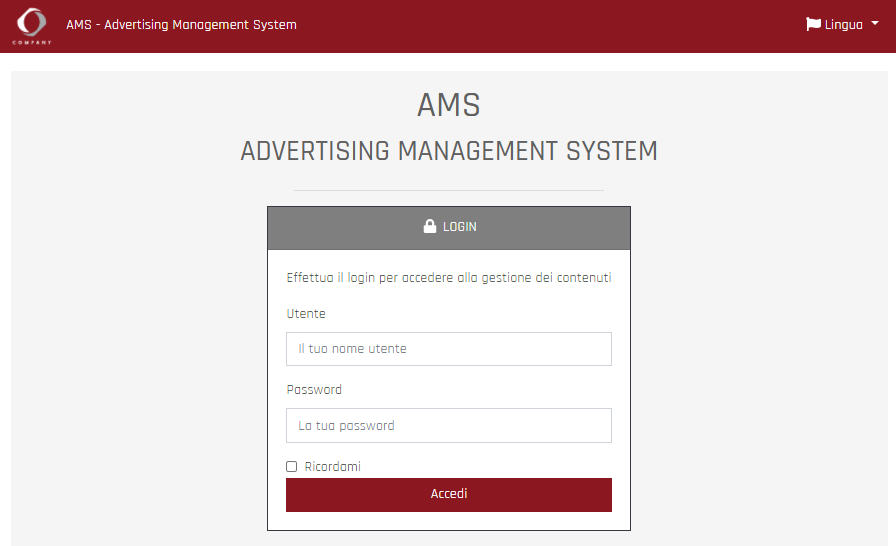
\includegraphics[width=0.95\textwidth]{login}
    \caption{Schermata di login}
    \label{fig:figure20}
    \end{center}
\end{figure}

\subsection{Scelta funzionalità}
La schermata principale del prodotto è la schermata di scelta funzionalità. Tramite questa schermata si possono raggiungere le varie funzioni offerte dal prodotto.
\begin{figure}[h]
    \begin{center}
    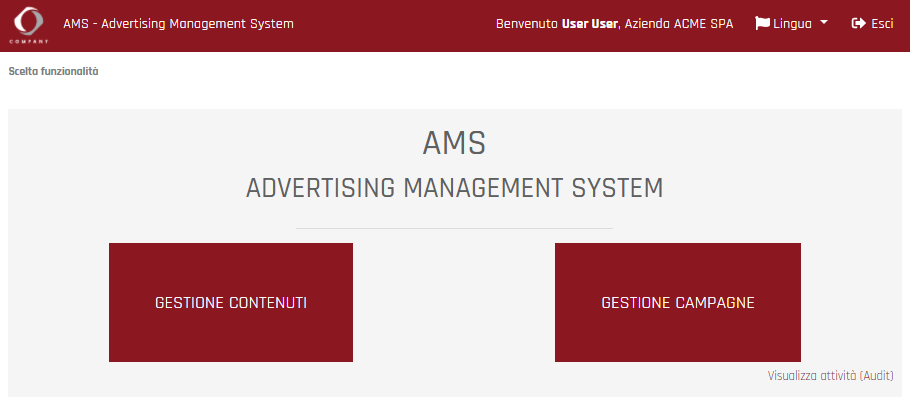
\includegraphics[width=1\textwidth]{funzionalita}
    \caption{Schermata di scelta funzionalità}
    \label{fig:figure21}
    \end{center}
\end{figure}
\\Più nello specifico le funzionalità raggiungibili tramite questa schermata sono:
\begin{itemize}
    \item gestione dei contenuti;
    \item gestione delle campagne (Non abilitata);
    \item visualizzazione \textit{audit}.
\end{itemize}

\subsection{Gestione contenuti}
Tramite la schermata di gestione contenuti è possibile raggiungere le sezioni di lavoro divise per ruolo (Editore, Redattore, Supervisore).
\begin{figure}[h]
    \begin{center}
    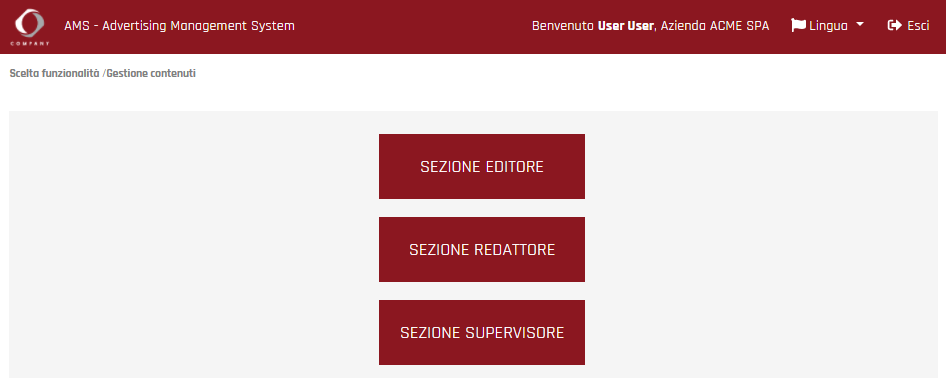
\includegraphics[width=1\textwidth]{gestcont}
    \caption{Schermata di gestione contenuti}
    \label{fig:figure22}
    \end{center}
\end{figure}
\\Ovviamente ogni utente puo visualizzare solamente le sezioni relative ai ruoli a lui assegnati.

\subsection{Sezione editore}
Questa sezione è quella in cui sono utilizzabili la maggior parte delle funzionalità obiettivo dello stage. In questa schermata è visualizzata una lista di tutti i \gls{contenutog}. Per ciascuno di questi è possibile:
\begin{itemize}
    \item visualizzarne l'anteprima;
    \item clonarlo;
    \item modificarlo;
    \item richiederne l'associazione;
    \item eliminarlo.
\end{itemize}
Nel caso sia stata richiesta l'associazione di un contenuto, questo non potra più essere eliminato né modificato.
Tramite questa pagina è inoltre possibile crearne uno nuovo.
\begin{figure}[h]
    \begin{center}
    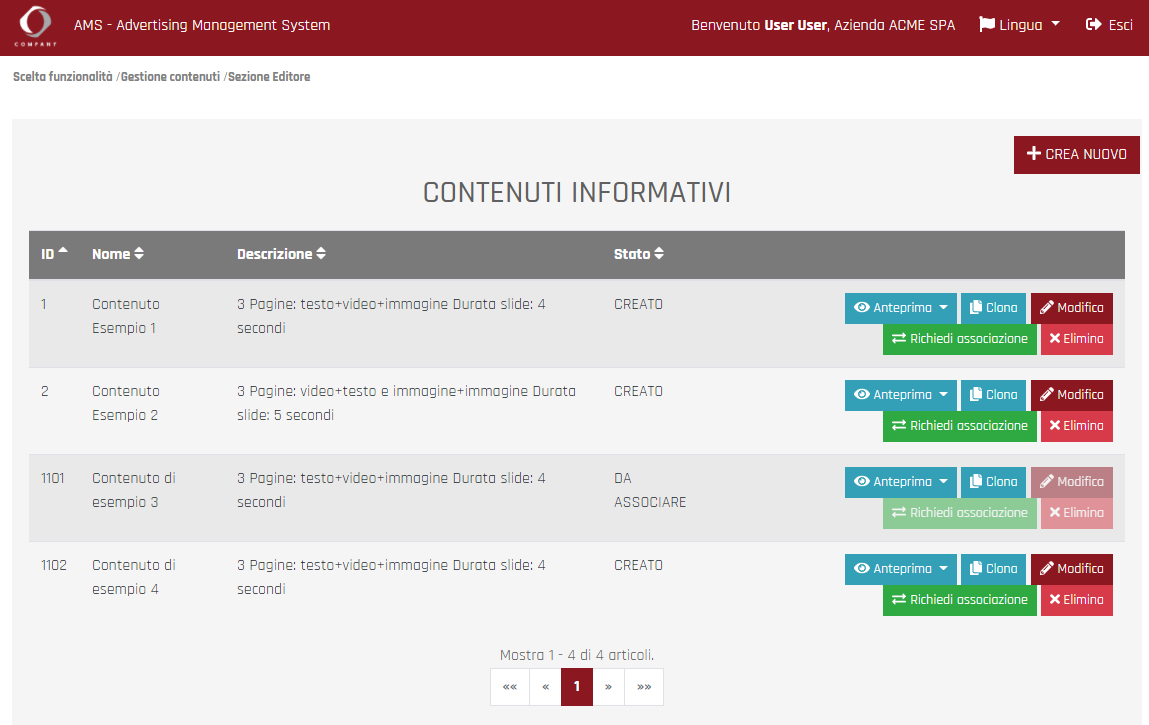
\includegraphics[width=1\textwidth]{editore}
    \caption{Schermata di gestione contenuti}
    \label{fig:figure23}
    \end{center}
\end{figure}

\subsection{Creazione di un contenuto}
La schermate di creazione di un contenuto è divisa in due aree. In quella di sinistra si inseriscono le informazioni generali relative al contenuto. In quella di destra è possibile creare le pagine del contenuto, selezionando per ciascuna uno tra i vari \textit{template} disponibili.
Nel caso si scelgano \textit{template} con contenuti multimediali è sufficiente che questi vengano caricati attraverso l'apposito pulsante. Nel caso ci siano contenuti testuali da inserire è possibile invece utilizzare l'apposito editor di testo.
\begin{figure}[h]
    \begin{center}
    \includegraphics[width=1\textwidth]{Creazione}
    \caption{Creazione di un contenuto}
    \label{fig:figure24}
    \end{center}
\end{figure}

\subsection{Anteprima di un contenuto}
La possibilità di visualizzare l'anteprima di un contenuto una volta creato è una delle funzionalità più utili e importanti. L'anteprima permette infatti di visualizzare come si presenterebbe un contenuto una volta pubblicato e permette di decidere se richiederne l'associazione o modificarlo.
\begin{figure}[h]
    \begin{center}
    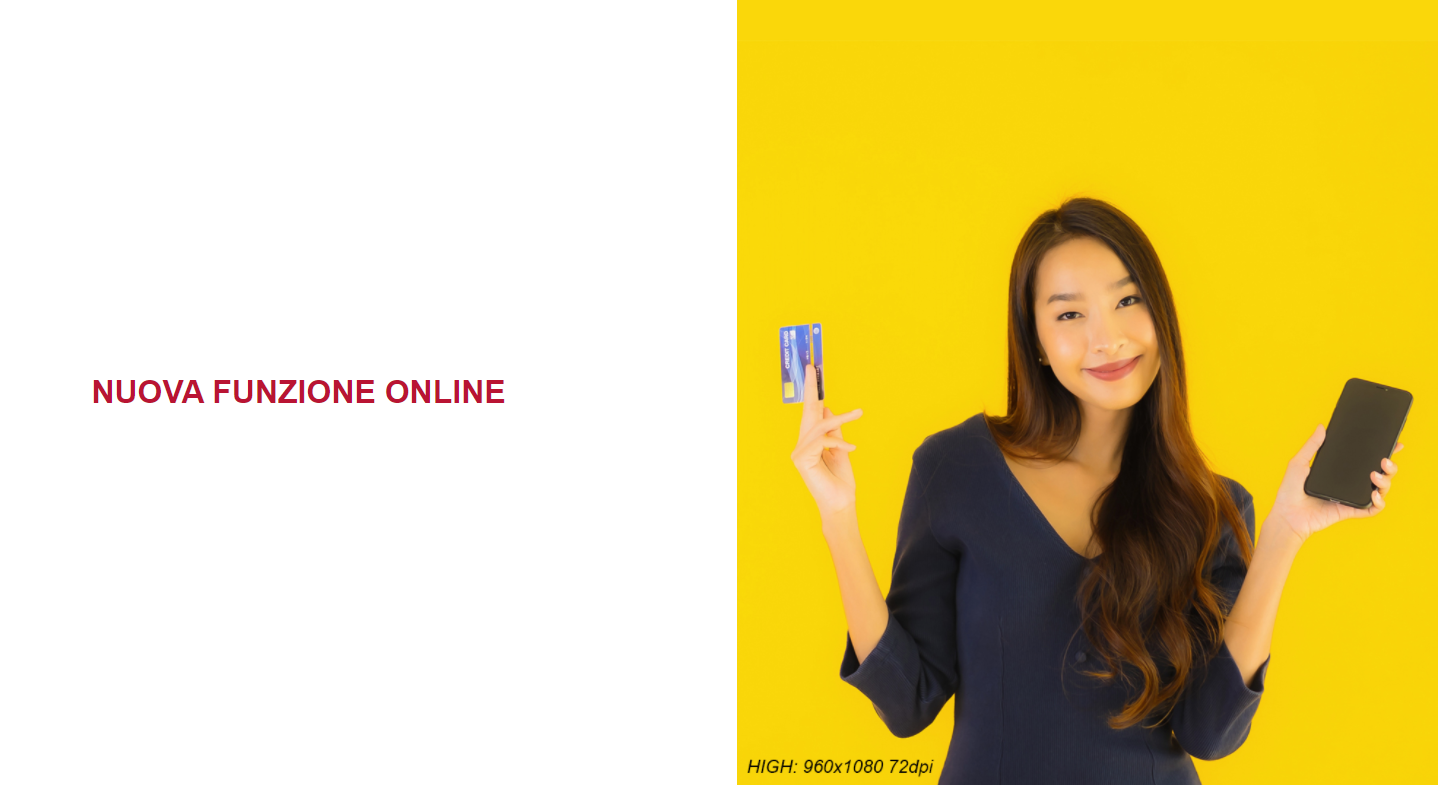
\includegraphics[width=1\textwidth]{anteprima}
    \caption{Anteprima di un contenuto di esempio}
    \label{fig:figure25}
    \end{center}
\end{figure}

\subsection{Clonazione di un contenuto}
La possibilità di clonare un contenuto è utile nel caso si voglia crearne uno simile ad uno già pubblicato senza la necessità di dover partire da zero. Per clonare un contenuto è sufficiente cliccare su \textit{"Clona"} nella sezione dedicata al ruolo di editore. Fatto ciò si aprirà automaticamente un pannello modale in cui è necessario inserire il nome che si vuole assegnare al nuovo contenuto.
\begin{figure}[h]
    \begin{center}
    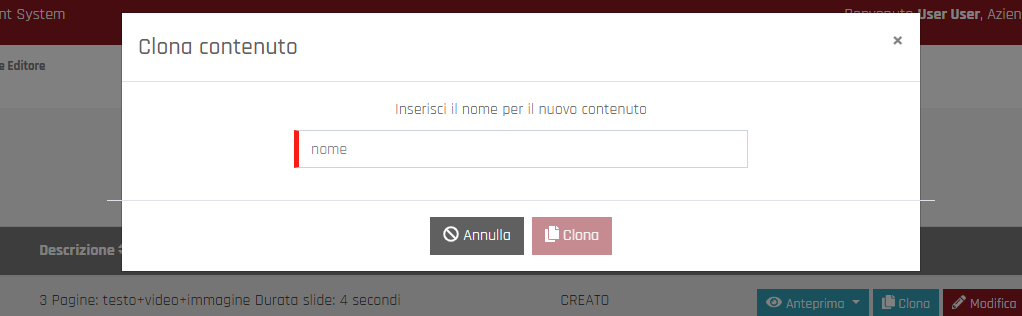
\includegraphics[width=1\textwidth]{clona}
    \caption{Clonazione di un contenuto}
    \label{fig:figure26}
    \end{center}
\end{figure}

\subsection{Modifica di un contenuto}
Modificare un contenuto può essere indispensabile nel caso, ad esempio, siano state inserite immagini o testi errati. La schermata di modifica di un contenuto si presenta in modo analogo a quella di creazione, con la differenza che i campi dati hanno già le informazioni del contenuto al loro interno.
\begin{figure}[h]
    \begin{center}
    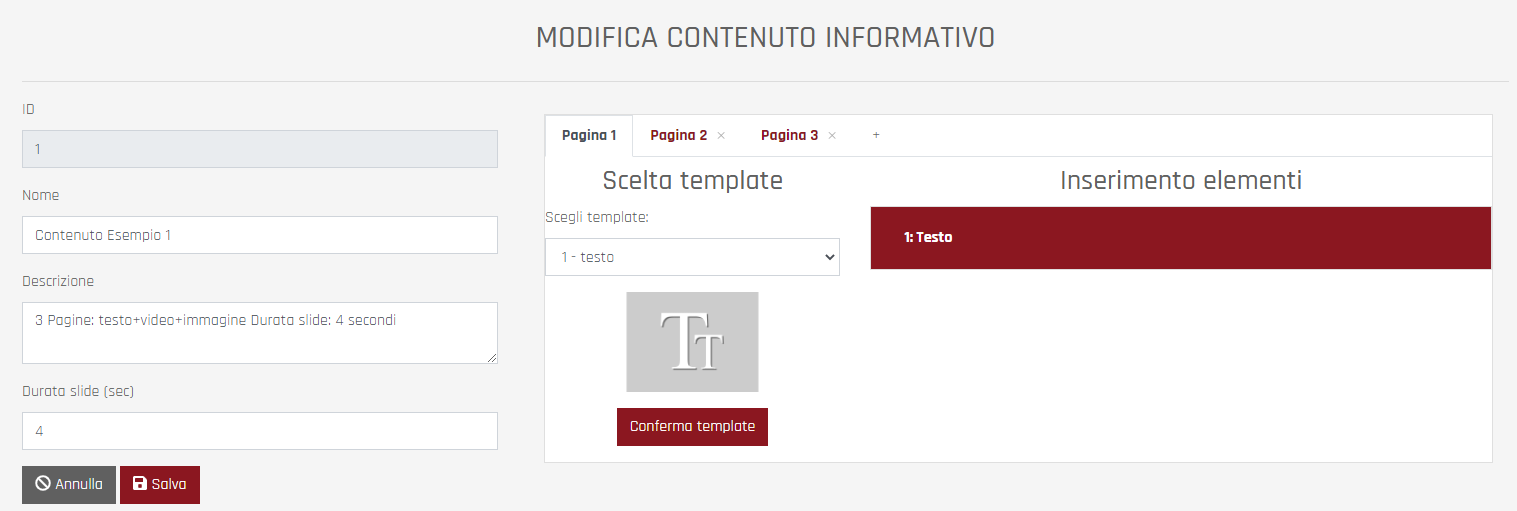
\includegraphics[width=1\textwidth]{modifica}
    \caption{Modifica di un contenuto}
    \label{fig:figure27}
    \end{center}
\end{figure}
\newpage
\subsection{Associazione di un contenuto}
La richiesta di associazione di un contenuto è il primo passo da eseguire perchè questo possa essere pubblicato. Una volta inoltrata la richiesta di associazione di un contenuto questo non potrà più essere modificato ne eliminato. L'associazione può essere approvata o rifiutata da un redattore; nel primo caso il contenuto potrà proseguire nel suo ciclo di vita, nel secondo tornerà allo stato iniziale e sarà di nuovo modificabile.
\begin{figure}[h]
    \begin{center}
    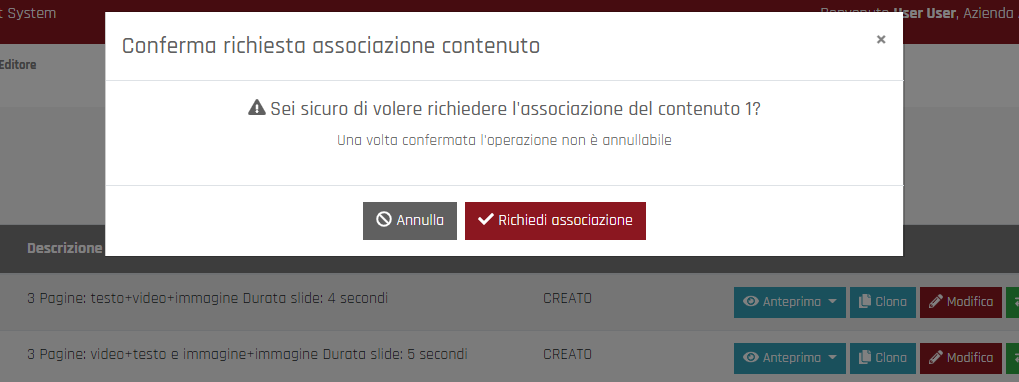
\includegraphics[width=1\textwidth]{associazione}
    \caption{Richiesta di associazione di un contenuto}
    \label{fig:figure28}
    \end{center}
\end{figure}

\subsection{Eliminazione di un contenuto}
Un contenuto potrebbe essere creato per errore oppure non essere più necessario. In questo caso può tornare utile l'eliminazione. L'eliminazione è irreversibile.
\begin{figure}[h]
    \begin{center}
    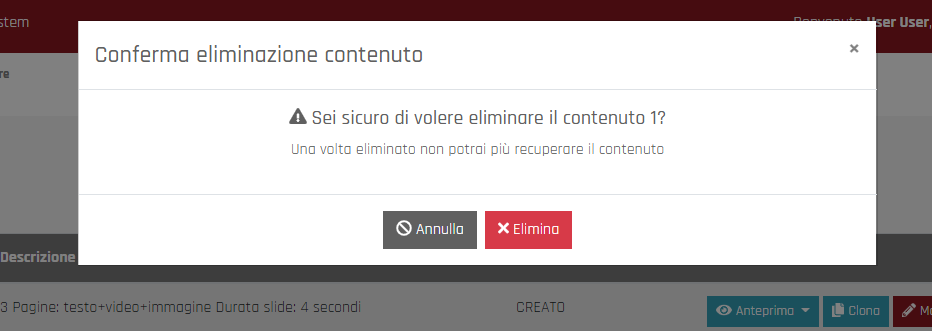
\includegraphics[width=1\textwidth]{eliminazione}
    \caption{Eliminazione di un contenuto}
    \label{fig:figure29}
    \end{center}
\end{figure}

\subsection{Audit}
La schermata di visualizzazione degli \textit{audit}, raggiungibile dalla schermata principale, è visualizzabile da chiunque abbia effetuato il \textit{Login} e raccoglie varie informazioni sulle attività effettuate dagli utenti.
\begin{figure}[h]
    \begin{center}
    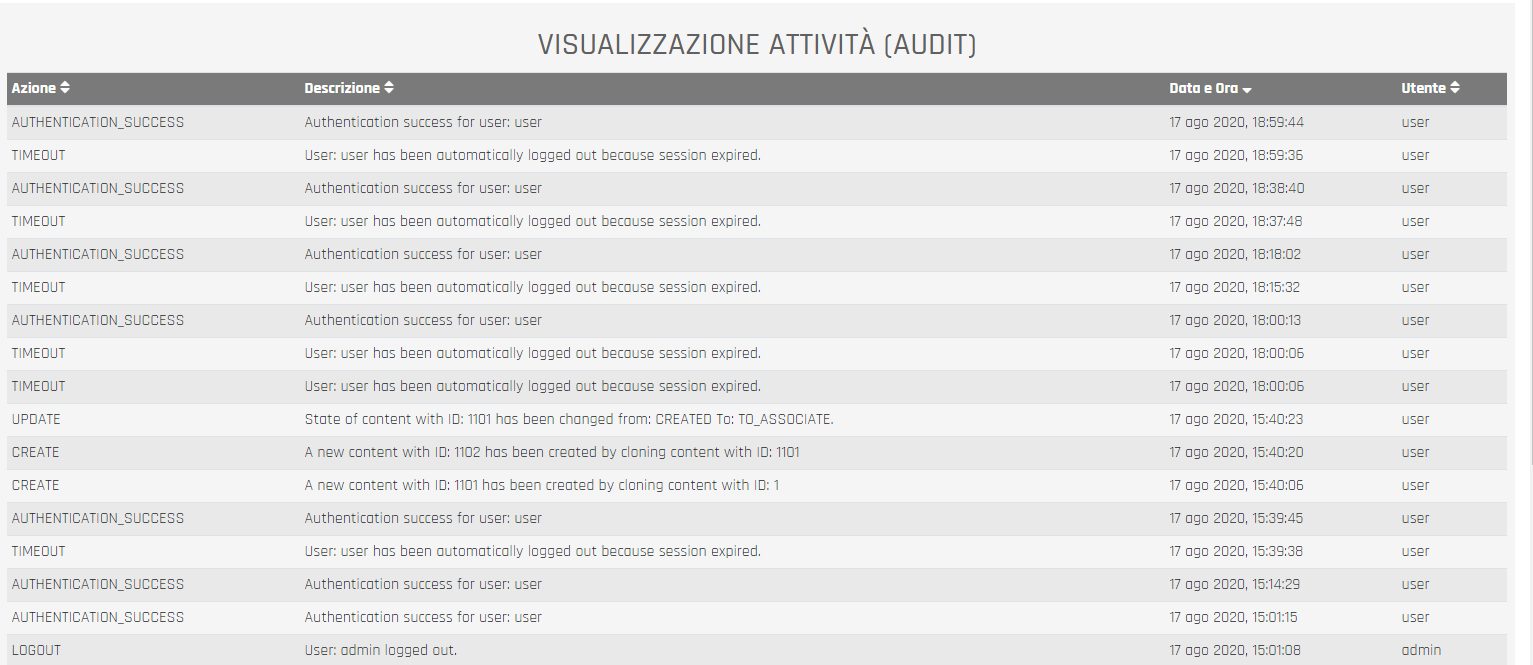
\includegraphics[width=1\textwidth]{audit}
    \caption{Visualizzazione audit}
    \label{fig:figure30}
    \end{center}
\end{figure}

%**************************************************************
\section{Documentazione}
Oltre allo sviluppo dell'applicazione vera e propria, una parte delle ore a disposizione è stata dedicata alla documentazione. In accordo con il \textit{Product Owner} è stato deciso di redigere solamente il manuale utente e il manuale sviluppatore.

\subsection{Manuale Utente}
Lo scopo di questo documento è illustrare tutte le funzionalità del prodotto. In tal modo l'utente finale ha a disposizione tutte le informazioni per utilizzare il \textit{software} correttamente.
Il manuale utente descrive:
\begin{itemize}
    \item requisiti di sistema;
    \item utilizzo dell'applicazione.
\end{itemize}

\subsection{Manuale Sviluppatore}
Lo scopo di questo documento è illustrare le scelte implementative effettuate durante lo sviluppo e dare informazioni utili ad uno sviluppatore che comincia a lavorare a questo progetto.
Il manuale sviluppatore tuttavia non ha lo scopo di sostituirsi alla documentazione ufficiale delle tecnologie utilizzate. Per tale motivo all'interno di esso sono contenuti numerosi riferimenti a documenti esterni.
Il manuale sviluppatore descrive:
\begin{itemize}
    \item setup dell'ambiente di lavoro;
    \item gestione delle dipendenze \textit{Angular};
    \item gestione della dipendenza ad \textit{Oracle};
    \item utilizzo di \textit{Angular CLI};
    \item \textit{build} e \textit{packaging} dell'applicazione;
    \item \textit{testing};
    \item utilizzo di \textit{Docker};
    \item \gls{ci};
    \item scelte implementative effettuate.
\end{itemize}

%**************************************************************
\section{Test}
Nello sviluppo di un'applicazione il \textit{testing} è una delle fasi più importanti. Poiché ogni due settimane veniva presentata una demo dell'applicativo, i \textit{test} sono stati eseguiti di continuo durante lo sviluppo, sia in modo automatico sia manualmente. \\Nel corso di questa sezione vengono descritti i \textit{test} svolti durante lo sviluppo.

\subsection{Test di unità}
I \textit{test} di unità sono eseguiti per verificare se sono presenti errori nei singoli metodi. Nel corso dello stage i \textit{test} di unità sono stati eseguiti tramite \textit{JUnit} e \textit{Jest}. Tali \textit{framework} sono sviluppati rispettivamente per \textit{Java} e per \textit{Javascript}. Il primo è stato utilizzato per testare il \textit{back-end} mentre il secondo per il \textit{front-end}.

\begin{lstlisting}[caption={Test di unità in Java},label={utj}]
    @Test
    @Transactional
    public void createContent() throws Exception {
        int databaseSizeBeforeCreate = contentRepository.findAll().size();
        // Create the Content
        restContentMockMvc.perform(post("/api/contents")
            .contentType(MediaType.APPLICATION_JSON)
            .content(TestUtil.convertObjectToJsonBytes(content)))
            .andExpect(status().isCreated());

        // Validate the Content in the database
        List<Content> contentList = contentRepository.findAll();
        assertThat(contentList).hasSize(databaseSizeBeforeCreate + 1);
        Content testContent = contentList.get(contentList.size() - 1);
        assertThat(testContent.getName()).isEqualTo(DEFAULT_NAME);
        assertThat(testContent.getState()).isEqualTo(DEFAULT_STATE);
        assertThat(testContent.getDescription()).isEqualTo(DEFAULT_DESCRIPTION);
        assertThat(testContent.getSlideTime()).isEqualTo(DEFAULT_SLIDE_TIME);
    }
\end{lstlisting}
\newpage
\begin{lstlisting}[caption={Test di unità in JavaScript},label={utj}]
    describe('Component Tests', () => {
  describe('Home Component', () => {
    let comp: HomeComponent;
    let fixture: ComponentFixture<HomeComponent>;
    let accountService: AccountService;
    let loginModalService: LoginModalService;

    beforeEach(async(() => {
      TestBed.configureTestingModule({
        imports: [AmsTestModule],
        declarations: [HomeComponent],
      })
        .overrideTemplate(HomeComponent, '')
        .compileComponents();
    }));

    beforeEach(() => {
      fixture = TestBed.createComponent(HomeComponent);
      comp = fixture.componentInstance;
      accountService = TestBed.get(AccountService);
      loginModalService = TestBed.get(LoginModalService);
    });

    it('Should call accountService.getAuthenticationState on init', () => {
      // WHEN
      comp.ngOnInit();

      // THEN
      expect(accountService.getAuthenticationState).toHaveBeenCalled();
    });

    it('Should call accountService.isAuthenticated when it checks authentication', () => {
      // WHEN
      comp.isAuthenticated();

      // THEN
      expect(accountService.isAuthenticated).toHaveBeenCalled();
    });

    it('Should call loginModalService.open on login', () => {
      // WHEN
      comp.login();

      // THEN
      expect(loginModalService.open).toHaveBeenCalled();
    });
  });
});
\end{lstlisting}

\subsection{Test di integrazione}
I \textit{test} di integrazione vengono eseguiti per verificare che non ci siano errori di integrazione tra le varie componenti del sistema. Nel corso del progetto questa fase di \textit{test} è stata ritenuta di grande importanza, in particolare nell'integrazione tra il \textit{back-end} e il \textit{front-end}. In questo caso i suddetti \textit{test} sono stati eseguiti manualmente. 

\subsection{Test di sistema}
I \textit{test} di sistema vengono eseguiti per assicurare che il sistema soddisfi i requisiti richiesti. \\Nel corso dello stage dopo l'implementazione di una nuova funzionalità l'intero sistema veniva testato. Al termine di ogni sprint tali \textit{test} venivano eseguiti dal \textit{product owner}, in tal caso questi possono essere considerati \textit{test} di accettazione.

\subsection{Test di performance}
I \textit{test} di performance vengono eseguiti per controllare che il sistema non risulti lento durante il suo utilizzo. Tali \textit{test} sono stati eseguiti con l'ausilio del pannello amministratore generato da \textit{JHipster}. Questo permette di visualizzare una moltitudine di informazioni, come ad esempio le risorse occupate o il tempo di esecuzione delle \gls{apig}.
\begin{figure}[h]
    \begin{center}
    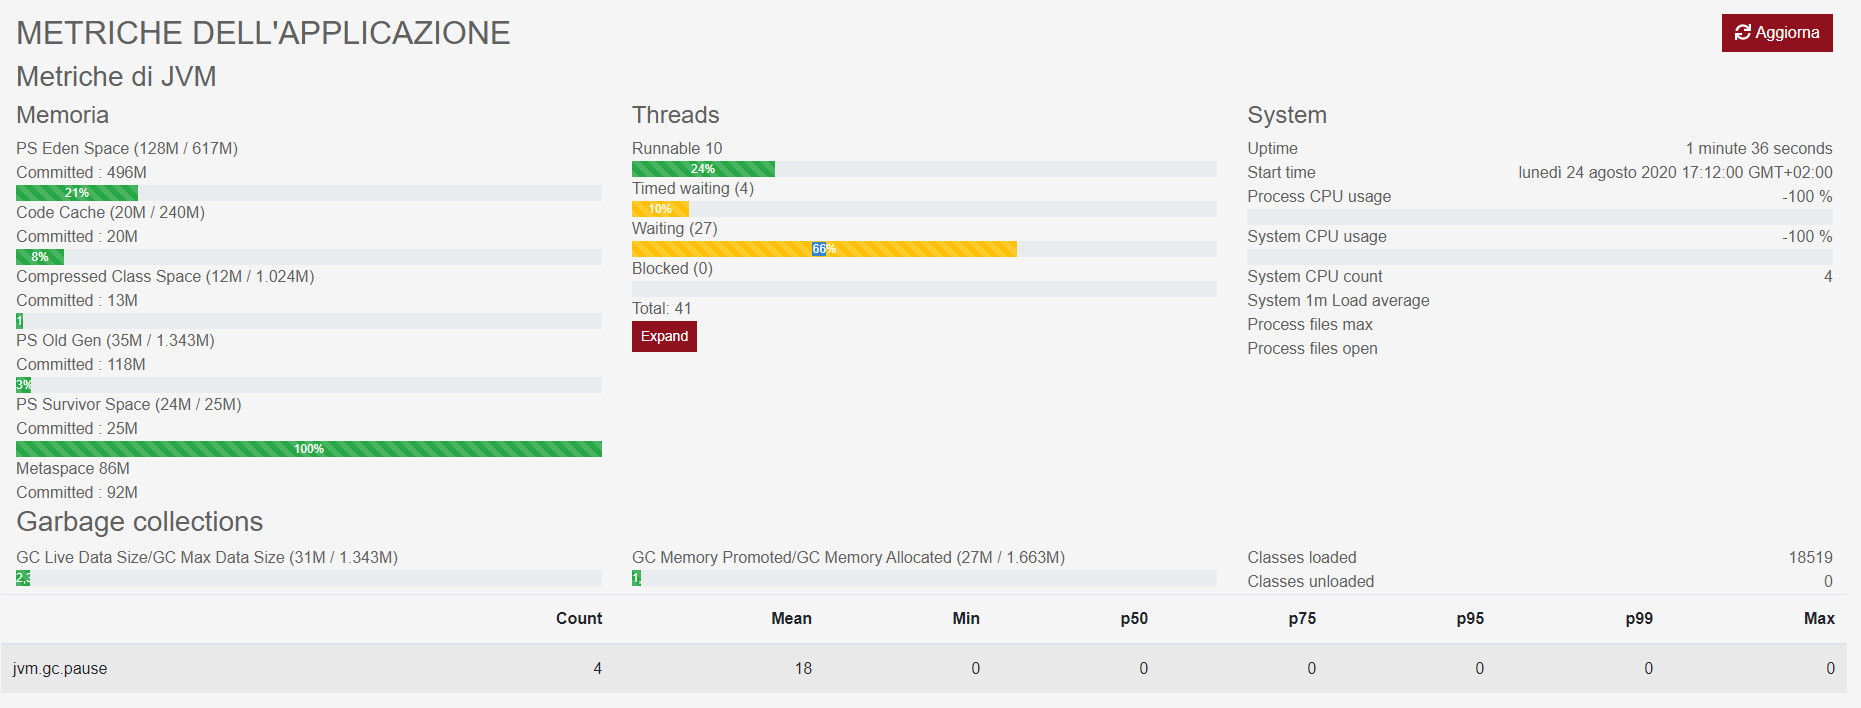
\includegraphics[width=1\textwidth]{metriche1}
    \caption{Metriche dell'applicazione}
    \label{fig:figure31}
    \end{center}
\end{figure}

\section{Accessibilità}
I \textit{test} di accessibilità sono necessari per verificare che l'applicativo risulti utilizzabile anche da utenti con disabilità. Nel corso del progetto si è cercato di attenersi alle regole definite nello standard \href{https://www.w3.org/TR/WCAG21/}{WCAG 2.1}. I test veri e propri sono stati poi eseguiti tramite \href{https://developers.google.com/web/tools/lighthouse/?utm_source=devtools}{\textit{Lighthouse}}, un tool per l'analisi dinamica di pagine web.             
% !TEX encoding = UTF-8
% !TEX TS-program = pdflatex
% !TEX root = ../tesi.tex

%**************************************************************
\chapter{Considerazioni finali}
\label{cap:considerazioni}
%**************************************************************

\intro{In questo capitolo sono esposte le considerazioni finali sul lavoro svolto corredate da una valutazione personale sullo stage.}\\

%**************************************************************
\section{Soddisfacimento degli obiettivi}
\subsection{Obiettivi obbligatori}
\begin{itemize}
    \item Ob1: soddisfatto. Ho imparato informazioni di base e non sull'utilizzo e il funzionamento di \textit{Spring}. Inoltre ho capito il funzionamento di \textit{Spring MVC REST} anche grazie al confronto diretto col tutor aziendale;
    \item Ob2: soddisfatto. Il \textit{database oracle} è stato implementato e ho compreso come interagirci. Ho anche avuto la possibilità di evidenziare le differenze di \textit{Oracle} rispetto ad altri \gls{dbmsg} di tipo relazionale;
    \item Ob3: Tutte le funzionalità di \textit{back-end} richieste sono state implementate e testate. Il prodotto finale consente infatti di eseguire tutte le operazioni evidenziate nell'analisi funzionale.
\end{itemize}
\subsection{Obiettivi desiderabili}
\begin{itemize}
    \item D1: soddisfatto. Il \textit{front-end} del prodotto è stato implementato e testato. Il \textit{front-end} è correttamente integrato con il \textit{back-end};
    \item D2: soddisfatto. \textit{Angular} è stato utilizzato per tutto lo sviluppo del \textit{front-end}. Ho avuto modo di vedere come utilizzare le librerie di \textit{Angular} e come modificare la presentazione di una pagina;
    \item D3: soddisfatto. Il \textit{team} di sviluppo è stato ritenuto autonomo e proattivo da parte dei rispettivi tutor aziendali.
\end{itemize}
\subsection{Obiettivi opzionali}
\begin{itemize}
    \item Op1: parzialmente soddisfatto. Ho avuto modo di comprendere il funzionamento e l'utilità di un processo di \gls{ci}/\gls{cd}. Ho capito il funzionamento della \textit{pipeline} di \gls{ci}/\gls{cd} presente nella \textit{repository} su \textit{GitLab} tuttavia non ho avuto modo di implementarne una da zero.
\end{itemize}

\section{Conoscenze acquisite}
Di seguito verranno elencate le conoscenze acquisite per ciascuna delle tecnologie utilizzate nel progetto e descritte nelle sezioni \ref{techs} e \ref{strum}.

\subsection{JHipster}
\textit{JHipster} è stato utilizzato come base di partenza per la creazione dell'applicazione. Nello specifico ho imparato a:
\begin{itemize}
    \item generare applicazioni con \textit{JHipster};
    \item importare un modello di database in un applicazione autogenerata;
    \item gestire i problemi legati all'aggiunta di nuove entità nel \textit{database};
    \item conoscere l'architettura definita dai programmatori di \textit{JHipster}.
\end{itemize}

\subsection{Java Enterprise}
Il \textit{back-end} dell'applicazione è interamente scritto in \textit{Java}. Nel corso dello stage ho potuto apprendere:
\begin{itemize}
    \item costrutti avanzati di \textit{Java};
    \item utilizzo di nuove librerie per lo sviluppo di applicazioni web;
    \item utilizzo di richieste \textit{multipart} per gestire il caricamento di elementi multimediali;
    \item scrittura di codice \textit{Java} più leggibile.
\end{itemize}

\subsection{Spring}
L'utilizzo di \textit{Spring} è stato fondamentale per lo sviluppo dell'applicazione. Durante lo sviluppo gli argomenti trattati sono stati i seguenti:
\begin{itemize}
    \item utilizzo di \textit{Spring} \textit{MVC} per separare la logica dalla presentazione;
    \item utilizzo di \textit{Spring} data per facilitare l'interazione con il database e garantire la transazionalità delle operazioni;
    \item utilizzo di \textit{Spring} \textit{boot} in modo da avviare l'applicazione all'interno del container \textit{Spring}, senza necessità di configurare un \textit{web server};
    \item funzionalità core di \textit{Spring};
\end{itemize}

\subsection{Hibernate}
\textit{Hibernate} ha facilitato di molto l'interazione col \textit{database}, è stato infatti utilizzato per:
\begin{itemize}
    \item mappare le entità definite in \textit{Java} come tabelle su \textit{Oracle};
    \item gestire \textit{query} effettuate ottenendo come risposta un oggetto \textit{Java};
    \item gestire la conversione dei campi dati da quelli utilizzati da \textit{Java} a quelli utilizzati da \textit{Oracle}.
\end{itemize}

\subsection{Rest}
Le \gls{apig} sono state definite seguendo il modello definito da \textit{REST}.
Durante la codifica delle \gls{apig} ho avuto modo di:
\begin{itemize}
    \item comprendere meglio le differenze tra i metodi \textit{HTTP (GET, PUT, POST, PATCH, DELETE)};
    \item definire \gls{apig} \textit{RESTful};
    \item evitare e prestare più attenzione ai problemi di sicurezza legati alla logica del codice scritto;
    \item scrivere codice che termina \textit{"gracefully"}, ovvero che anche in caso di errori gravi non causa interruzioni al sistema.
\end{itemize}

\subsection{Oracle}
Durante l'implemetazione di \textit{Oracle} sono stati trattati diversi argomenti, alcuni non direttamente correlati col \textit{database} stesso ma comunque degni di nota. Più nello specifico:
\begin{itemize}
    \item aggiunta e utilizzo dei driver \textit{Oracle} a un progetto \textit{Java};
    \item studio delle differenze tra \textit{Oracle} e altri \gls{dbmsg};
    \item configurazione e utilizzo di una \textit{VPN} per l'accesso all'intranet aziendale.
\end{itemize}

\subsection{Liquibase}
\textit{Liquibase} ha permesso di gestire in modo semplice ed efficace le modifiche allo schema del \textit{database}. Durante lo stage ho imparato a:
\begin{itemize}
    \item modificare manualmente i \textit{changelog} di \textit{Liquibase};
    \item inserire nuove entità e relazioni nello schema;
    \item comprendere e risolvere conflitti nei \textit{changelog}.
\end{itemize}

\subsection{Angular}
Il \textit{front-end} di AMS è interamente scritto in \textit{Angular}. Gli argomenti trattati sono stati:
\begin{itemize}
    \item importazione e utilizzo di moduli \textit{Angular};
    \item modifiche all'interfaccia grafica;
    \item inserimento di traduzioni automatiche per gestire l'internazionalizzazione;
    \item integrazione di \gls{apig} RESTful con il \textit{front-end}.
\end{itemize}

\subsection{Eclipse}
Nonostante avessi già utilizzato \textit{Eclipse} in precedenza ho comunque acquisito nuove conoscenze di tale strumento, più nello specifico:
\begin{itemize}
    \item gestione di un progetto \textit{Maven} con \textit{Eclipse};
    \item \textit{debug} dell'applicazione.
\end{itemize}

\subsection{Maven}
La fase di \textit{build} del progetto è stata gestita interamente con \textit{Maven}.
Ho avuto modo di apprendere:
\begin{itemize}
    \item il funzionamento del \textit{file POM} per la gestione delle dipendenze;
    \item la \textit{build} dell'applicazione tramite \textit{Maven};
    \item l'esecuzione dei \textit{test} automatici tramite \textit{Maven};
\end{itemize}

\subsection{Git}
Per gestire il versionamento del \textit{software} è stata utilizzata una \textit{repository} su \textit{GitLab}. Durante lo sviluppo è stato necessario apprendere al meglio l'utilizzo di \textit{GIT} per gestire il versionamento e i conflitti, più nello specifico:
\begin{itemize}
    \item utilizzo di \textit{GIT} da linea di comando;
    \item utilizzo del \gls{fbwg}\glsfirstoccur{};
    \item gestione dei conflitti durante il \textit{merge};
    \item rilascio di una nuova versione del \textit{software}.
\end{itemize}

\subsection{SQLDeveloper}
Durante il corso del progetto questo strumento è stato utilizzato per:
\begin{itemize}
    \item verificare che i dati fossero inseriti correttamente nel \textit{database};
    \item verificare che le \textit{query} sul \textit{database} restituissero il risultato aspettato.
\end{itemize}

\section{Valutazione finale}
Sono molto contento dell'esperienza fatta durante il periodo di stage. Ho avuto la possibilità di lavorare all'interno di un azienda assieme ad un \textit{team} di lavoro composto da un altro stagista e dai due tutor. Questo ha favorito l'apprendimento di competenze tecniche e, soprattutto, ha migliorato la mia capacità di lavorare in gruppo in un contesto lavorativo. Per quanto riguarda il prodotto tutti gli obietivi prefissati sono stati completati e alla fine dello stage è stata fatta una presentazione del prodotto al direttore. La presentazione è andata bene e tutte le funzionalità richieste sono state mostrate, al termine di essa ci sono state fatte alcune domande con una modalità simile a un colloquio. Qualche giorno dopo sono stato nuovamente contattato dall'azienda che mi ha fatto una proposta di assunzione, spronandomi prima a terminare gli studi. Questo mi ha reso molto fiero del lavoro svolto, reputo quindi questa esperienza del tutto positiva.                                          

%**************************************************************
% Materiale finale
%**************************************************************
\backmatter
\printglossaries
% !TEX encoding = UTF-8
% !TEX TS-program = pdflatex
% !TEX root = ../tesi.tex

%**************************************************************
% Bibliografia
%**************************************************************

\cleardoublepage
\chapter{Bibliografia}

\nocite{*}
% Stampa i riferimenti bibliografici
\printbibliography[heading=subbibliography,title={Riferimenti bibliografici},type=book]

% Stampa i siti web consultati
\printbibliography[heading=subbibliography,title={Siti web consultati},type=online]


\end{document}
